\documentclass[11pt,a4paper]{article}
\usepackage{url}
\usepackage{cite}
\usepackage{longtable}
\usepackage{graphicx}

\setlength{\parindent}{0mm}
\setlength{\oddsidemargin}{0mm}
\setlength{\oddsidemargin}{0mm}
\setlength{\topmargin}{0mm}
\setlength{\textheight}{245mm}
\setlength{\textwidth}{165mm}
\setlength{\headheight}{0mm}
\setlength{\headsep}{0mm}
\setlength{\parskip}{3mm}

\usepackage{bookmark,hyperref}

\hypersetup{
%     bookmarks=true,         % show bookmarks bar?
    unicode=true,          % non-Latin characters in Acrobat’s bookmarks
    pdftoolbar=true,        % show Acrobat’s toolbar?
    pdfmenubar=true,        % show Acrobat’s menu?
    pdffitwindow=false,     % window fit to page when opened
    pdfstartview={FitH},    % fits the width of the page to the window
    pdftitle={HHblits/HHsearch User Guide},      % title
    pdfauthor={Michael Remmert, Johannes Soeding},  % author
    pdfsubject={Userguide},   % subject of the document
    pdfnewwindow=true,      % links in new window
    colorlinks=true,        % false: boxed links; true: colored links
     linkcolor=black,        % color of internal links
     citecolor=black,        % color of links to bibliography
%     filecolor=black,        % color of file links
%     urlcolor=black,         % color of external links
}
%\urlstyle{same}            % show urls using the same font as the text


%\title{Quick guide to HHsearch} 

\begin{document}
\bibliographystyle{dcu}
%\maketitle

\begin{center}

\vspace{30mm}
{\Huge Quick guide to HHblits/HHsearch}\\[2mm]
  Version 2.2.11 (May 2011)\\[2mm]
\copyright  Michael Remmert \& Johannes S\"oding\\[2mm]
For bug reports, questions, or comments please contact johannes@soeding.com
\end{center}

{\noindent HHblits/HHsearch is a software suite for detecting remote homologues of proteins and generating high-quality alignments for homology modeling and function prediction. In addition to the command line package described here, there are two web server (HHblits, HHpred) available at \url{http://toolkit.tuebingen.mpg.de} or \url{http://toolkit.lmb.uni-muenchen.de} that runs the HHblits/HHsearch software and offers extended interactive functionality such as checking query and template alignments, histogram views of alignments, building 3D models with MODELER etc. The performance of this software suite is testified by the fact that in the latest CASP competition (2010) a fully automated version was assessed as one of the best out of the 81 servers, in particular in template-based structure prediction, the category most relevant for biological applications. (\url{http://predictioncenter.org/casp9/groups_analysis.cgi?type=server&tbm=on&submit=Filter}) Remarkable is that with $\sim 4$ minutes median response time, HHpred is about 100 faster than other top servers. Similar results could be achived in the previous rounds of CASP [Hildebrand A \emph{et al.} (2009) \emph{Proteins} {\bf 77}, 128-132. Battey JND \emph{et al.} (2007) \emph{Proteins} {\bf 69}, 68-82].}

\newpage

\setlength{\parskip}{0mm}
\tableofcontents
\setlength{\parskip}{2mm}

\newpage

\section{Obtaining HHblits and the databases}

Binaries can be downloaded for Linux x86 (32bit), Linux AMD64, and Apple PPC OS X can be downloaded at
\begin{verbatim}
  ftp://toolkit.lmb.uni-muenchen.de/HHblits/
\end{verbatim}

In the subdirectory \verb`databases/` different databases can be downloaded:
\small 
\begin{verbatim}
 1 NR20       (c) Remmert & Soeding, based on NR, clustered to 20 % sequence identity
 2 UniProt20  (c) Remmert & Soeding, based on UniProt, clustered to 20 % sequence identity
\end{verbatim} 
\normalsize

All databases consists of an HMM database, an A3M database and a database for prefiltering.

\section{Obtaining HHsearch and the databases}

Binaries can be downloaded for Linux x86 (32bit), Linux AMD64, Windows x86 (now includes multi-threading support),
Apple PPC OS X, and SUN Solaris can be downloaded at
\begin{verbatim}
  ftp://ftp.tuebingen.mpg.de/pub/protevo/HHsearch/
\end{verbatim}

In the subdirectory \verb`databases/` many databases can be downloaded:
\small 
\begin{verbatim}
 1* pdb70       (c) J. Soeding, based on PDB, updated weekly
 2* scop70      (c) J. Soeding, based on SCOP, updated with SCOP
 3* PfamA       http://www.sanger.ac.uk/Software/Pfam/
 4* SMART       http://smart.embl-heidelberg.de/}, downloaded from NCBI site
 5* PfamB       based on ProDom, downloaded from Pfam site
 6* COG         http://www.ncbi.nlm.nih.gov/COG/new/
 7* KOG	        http://www.ncbi.nlm.nih.gov/COG/new/
 8* CD/NCBI     http://www.ncbi.nlm.nih.gov/Structure/cdd/cdd.shtml
 9  Panther     http://www.pantherdb.org/, from InterPro
10  TIGRFAMs    http://tigrblast.tigr.org/web-hmm/, from InterPro
11  PIRSF       http://pir.georgetown.edu/pirsf/, from InterPro
12  Superfamily http://supfam.mrc-lmb.cam.ac.uk/SUPERFAMILY/, from InterPro
13  CATH/Gene3D http://cathwww.biochem.ucl.ac.uk/latest/, from InterPro 
\end{verbatim} 
\normalsize

The eight databases marked by an asterisc can be downloaded with HMMs in HHsearch 
format (*.hhm.tar files) and the\emph{multiple sequence alignments (MSAs)} in 
A3M format (*.a3m.tar files). The *.hhm.tar and *.a3m.tar files untar into thousands
of separate files, so before unnzipping and untarring, first create a directory for 
the database. Note that you can transform all A3M files to FASTA by using the 
\verb`reformat.pl` script supplied with HHsearch:
\begin{verbatim}
  > ./reformat.pl '*.a3m' .fas
\end{verbatim}

For the other five databases, you can download the HMM models in HMMer format as 
*.hmm.tar files. The *.hmm.tar files untar into a single concatenated HMMer file. 
For theses databases, unfortunately no alignments are publicly available (info to the 
contrary is wellcome.) 


\section{Getting started}

\subsection{Overview of programs}

\small 
\begin{verbatim}
  hhmake         Build an HMM from an input MSA in A2M, A3M, or FASTA format 
  hhblits        Iteratively search a database of HMMs with a query sequence or alignment
  hhsearch       Search a database of HMMs with a query MSA or HMM
  hhalign        Pairwise alignment of two HMMs/MSAs, dot plots etc.
  hhfilter       Filter MSA by maximum sequence identity, coverage, etc.  
  reformat.pl    Reformat one or many MSAs
  buildali.pl    Build a PSI-BLAST MSA from a sequence or MSA, add sec. structure
  addss.pl       Add secondary structure information to a given MSA
  alignhits.pl   Extract an MSA from a BLAST/PSI-BLAST output
  hhmakemodel.pl Generate MSAs or coarse 3D models from HHsearch results file	
  Align.pm       Perl package for local and global sequence-sequence alignment
\end{verbatim} 
\normalsize

Call a program without arguments (or with -h) to get a more detailed description of 
its syntax.


\subsection{Search with a query sequence through a database and generate a MSA}

The best way to generate a MSA (Multiple Sequence Alignment) is to use the HHblits software 
from this package. HHblits performs an iterative HMM-HMM comparison and has a runtime comparable 
to that of PSI-BLAST. This runtime is achived by a fast profile-profile prefilter based on SSE2 
instructions, which reduces the number of comparisons in the time-consuming HMM-HMM comparison 
step.

The default parameters for HHblits can be adapted in the configuration file 
\verb`.hhdefaults`. This tool needs for running the path to the two needed libraries
(\verb`context_data.lib` and \verb`cs219.lib` in the \verb`libs/`-directory of this package) 
and the basename of the database (e.g. \verb`databases/uniprot20`). The following database files 
must be present:

\begin{verbatim}
  BASENAME.cs219                database for the prefiltering step
  BASENAME_hhm_db               HMM databases
  BASENAME_hhm_db.index         index table for HMM databases
\end{verbatim}

When performing more than 1 search iteration or if an MSA should be generated, you also need the 
following databases:

\begin{verbatim}
  BASENAME_a3m_db               A3M databases
  BASENAME_a3m_db.index         index table for A3M databases
\end{verbatim}

The database scan with HHblits can be started by typing:

\begin{verbatim}
  > ./hhblits -i query.seq -d databases/uniprot20
\end{verbatim}

The complete search results, including the pairwise query-template alignments, are written to 
the default output file, \verb`query.hhr`. If you are interested in the MSA, you have to add the 
\verb`-oa3m` option:

\begin{verbatim}
  > ./hhblits -i query.seq -d databases/uniprot20 -oa3m query_profile.a3m
\end{verbatim}

A special parameter \verb`mact` can be used to choose the tradeoff between sensitivity and 
precision. With a low mact-value (e.g. \verb`-mact 0.01`) you get very sensitive, but not 
so precise alignments, whereas a search with a high mact-value (e.g. \verb`-mact 0.9`) results 
in shorter, but very precise alignments. The default value of mact in HHblits is $0.5$. 

If everything works, you will obtain an A3M-formatted MSA in file query.a3m. The next step would 
be to add secondary structure information to this alignment. This can be done by using the script
\verb`addss.pl` (you have to fill in a few paths at the top of the script for needed binaries):

\begin{verbatim}
  > ./addss.pl query.a3m
\end{verbatim}

Now you can generate a hidden Markov model (HMM) from this MSA:
\begin{verbatim}
  > ./hhmake -i query.a3m
\end{verbatim}



Another way uses the script \verb`buildali.pl` from this package. It builds an A3M alignment 
with iterated PSI-BLAST. It checks after each round for each HSP (i.e. for each PSI-BLAST 
matched sequence fragment) if both its ends have a sufficiently high score per column 
(e.g. 1/6 bits/column) with the query sequence, or rather with a 'core profile' of sequences 
most similar to the query. It prunes the HSP ends that do not have sufficient similarity, 
thus largely suppressing the frequent problem of profile corruption coming from the ends of 
domains, coiled coil regions, or low complexity regions. In a representative all-against-all 
benchmark on SCOP20, \verb`buildali.pl` was able to reduce the number of high-scoring 
false-positives by a factor of approximately five, while only slightly reducing sensitivity 
for very remote homologs. \verb`buildali.pl` also automatically adds PSIPRED secondary structure 
prediction. 

To get \verb`buildali.pl` to run you have to fill in a few paths at the top of the script, 
for example to the BLAST directory, PSIPRED data and binaries directories etc. Some of 
the same paths also have to be inserted at the top of the script \verb`alignhits.pl` which 
is called by \verb`buildali.pl`. Finally, you need to have a non-redundant database like the 
nr from NCBI filtered to 90 and 70 percent (e.g. by using the program CD-HIT from 
Weizhong Lee, \url{http://cd-hit.org/}). You can call these databases nr90 and nr70, for 
example, and would set the \$dbbase variable to "some\_path/nr". The script then adds 
the "90" and "70" as needed. It will first search the nr90 until more than 50 
sequences are found, whence it will switch to the nr70. To test \verb`buildali.pl` you might 
as well set a link from the nr to nr90 and nr70, which means \verb`buildali.pl` will search 
the entire nr (which is slower and a little less sensitive). Then start \verb`buildali.pl` 
with your sequence:
\begin{verbatim}
  > ./buildali.pl query.seq
\end{verbatim}

If everything works, you will obtain an A3M-formatted MSA in file query.a3m 
as a result. (Make sure all paths are correct and your active shell is bash: 
\verb`ln -s /bin/bash /bin/sh.`)

Now you can generate a hidden Markov model (HMM) from this MSA:
\begin{verbatim}
  > ./hhmake -i query.a3m
\end{verbatim}


\subsection{Search with a profile HMM through a database}

For searching with a profile HMM as query, you can either use HHblits or HHsearch. HHblits
uses a prefilter and performs the HMM-HMM comparison only on a small subsets of HMMs that pass
this prefilter. Therefore, HHblits has a dramatical shorter runtime by a small decrease in 
sensitivity (see Figure \ref{fig:hhsearch_hhblits_bench}). 

\begin{figure}[t]
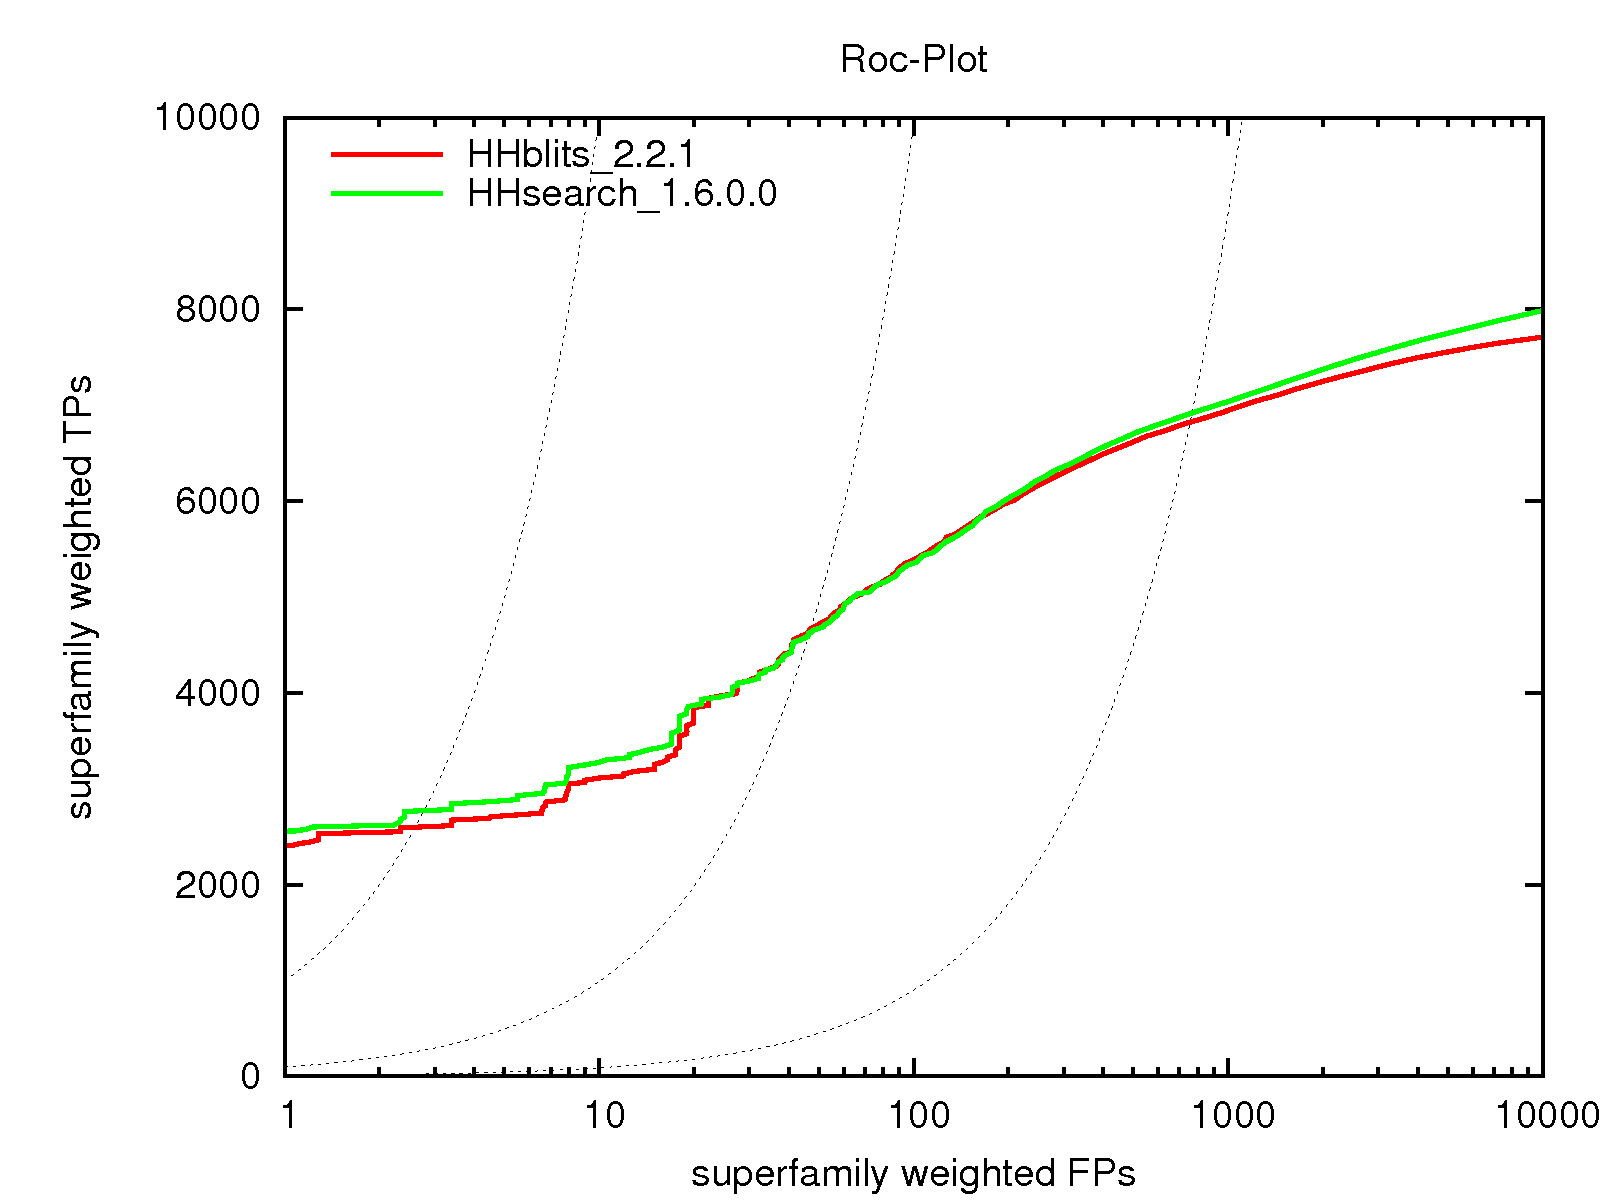
\includegraphics[width=\textwidth]{hhblits-hhsearch.png}
\caption{Benchmark of HHsearch and HHblits on a SCOP20 dataset.}
\label{fig:hhsearch_hhblits_bench}
\end{figure}

Using HHblits follows the same syntax as described in the previous section with an A3M-alignment
or an HMM-profile as input and a single iteration:

\begin{verbatim}
  > ./hhblits -i query_profile.a3m -d databases/uniprot20 -n 1
\end{verbatim}


To start using HHsearch, untar a database first, e.g.
\begin{verbatim}
  > cd scop70_1.72pre
  > tar -xzvf scop70_1.72pre.hhm.tar.gz
\end{verbatim}

The name \verb`scop70_1.72pre` stands for 'SCOP domain database version 1.72 (pre-SCOP) 
filtered to 70\% maximum sequence identity'.

Then, to generate a database file by concatenating all *.hhm files type (under LINUX)
\begin{verbatim}
  > cat *.hhm > scop70_1.72pre.hhm
\end{verbatim}

Test whether hhsearch works by typing
\begin{verbatim}
  > ./hhsearch -i d1hxn__.hhm -d scop70_1.72pre.hhm
\end{verbatim}

You should see a dot printed for every twenty HMMs processed until at the end 
hhsearch prints out a list with the best hits from the database. The complete 
search results, including the pairwise query-template alignments, are written to the 
default output file, \verb`d1hxn__.hhr`. The format (HH results format, HHR) was 
designed to be easily parsable.

Instead of using the hmm file you can also take the a3m file for the scan. It is 
automatically converted to an HMM by HHsearch before starting the scan:
\begin{verbatim}
  > ./hhsearch -i d1hxn__.a3m -d scop70_1.72pre.hhm
\end{verbatim}



\subsection{Building customized databases}

\subsubsection{HHblits databases}

If you want to build your own database from a set of sequences, call 
\begin{verbatim}
  >   ./hhblits -i <seqfile> -o /dev/null -oa3m <MSA-file>
\end{verbatim}

for every sequence in your database, as described in subsection 3.2. Default paramters 
are up to 2 search iterations at an E-value of 1E-3. These can be changed with the 
\verb`'-n <int>'` and \verb`'-e <float>'` options (Call \verb`hhblits` without parameters for a 
complete list of options). 

The next step is to add secondary structure prediction from PSIPRED (D. Jones, 1999) to the
MSA. This can be done by the script \verb`addss.pl` (When the sequence has a SCOP or PDB identifier as first word 
in its name, the script tries to add the DSSP states as well. You need to give the 
path to your local pdb or dssp directory for this to work.):

\begin{verbatim}
  >   ./addss.pl <MSA-file>
\end{verbatim}

Now you can use the two scripts \verb`create_cs_db.pl` and \verb`create_db.pl` to generate the
needed databases for HHblits. In both scripts you have to adapt some path at the beginning.

The first script \verb`create_cs_db.pl` generates the column state database needed for the 
prefilter step in HHblits. You can start it by typing:

\begin{verbatim}
  > ./create_cs_db.pl -i <MSA-dir> -o databases/DB.cs219
\end{verbatim}

The other script \verb`create_db.pl` generates the HMM- and A3M-databases:

\begin{verbatim}
  > ./create_db.pl -a3mdir <MSA-dir> -oa3m databases/DB_a3m_db -ohhm databases/DB_hhm_db
\end{verbatim}

A list of additional options for these scripts can be retrieved by calling the scripts without 
parameters.

\subsubsection{HHsearch databases}

If you want to build your own database from a set of sequences, call 
\begin{verbatim}
  >   ./hhblits -i <seqfile> -o /dev/null -oa3m <MSA-file>
\end{verbatim}

for every sequence in your database, as described in subsection 3.2. Default paramters 
are up to 2 search iterations at an E-value of 1E-3. These can be changed with the 
\verb`'-n <int>'` and \verb`'-e <float>'` options (Call \verb`hhblits` without parameters for a 
complete list of options). 

The next step is to add secondary structure prediction from PSIPRED (D. Jones, 1999) to the
MSA. This can be done by the script \verb`addss.pl` (When the sequence has a SCOP or PDB identifier as first word 
in its name, the script tries to add the DSSP states as well. You need to give the 
path to your local pdb or dssp directory for this to work.):

\begin{verbatim}
  >   ./addss.pl <MSA-file>
\end{verbatim}

Then generate an HHM file for each MSA by typing
\begin{verbatim}
  > ls | grep "\.a3m\$" | xargs hhmake -i 
\end{verbatim}

if your MSAs have extension a3m. You can then concatenate your individual HMMs
into your database:
\begin{verbatim}
  > cat *.hhm > yourDB.hhm
\end{verbatim}
(or, if maximum buffer size is exceeded, 
\begin{verbatim}
  > ls | grep "\.hhm\$" | xargs -i cat {} >> yourDB.hhm).
\end{verbatim}

By default, the option -M first will be used. This means that exactly those columns of 
the MSAs which contain a residue in the query sequence will be assigned to Match 
/ Delete states, the others will be assigned to Insert states. (The query sequence is 
the first sequence not containing secondary structure information.) Alternatively, you 
may want to apply the 50\%-gap rule by typing \verb`-M 50`, which assigns only those columns 
to Insert states which contain more than 50\% gaps. The \verb`-M first` option makes sense 
if your alignment can best be viewed as a seed sequence plus aligned homologs to 
reinforce it with evolutionary information. This is the case in the SCOP and PDB 
versions of our HMM databases, since here MSAs are built around a single seed 
sequence (the one with known structure). On the contrary, when your alignment 
represents an entire family of homologs and no sequence in particular, it is best to 
use the 50\% gap rule. This is the case for Pfam or SMART MSAs, for instance. 
Despite its simplicity, the 50\% gap rule has been shown to perform well in practice.

When calling hhmake, you may also apply several filters, such as maximum pairwise 
sequence identity (\verb`-id <int>`), minium sequence identity with query sequence 
(\verb`-qid <int>`), or miniumum coverage with query (\verb`-cov <int>`). But beware 
of making your MSAs too restrictive, as this will lower the sensitivity for remote homologs.


\subsection{Maximum Accuracy alignment algorithm}

HHblits and HHsearch use a better alignment algorithm than the quick and 
standard Viterbi method to generate the final HMM-HMM alignments. Both realign
all diplayed alignments in a second stage using the more accurate Maximum Accurracy 
(MAC) algorithm (Durbin, Eddy, Krough, Mitchison: Biological sequence analysis, page 
95; extension to HMM-HMM: Biegert, Lupas, and S\"oding (2008) \emph{Bioinformatics.} 
\textbf{24}, 807--814.). The Viterbi algorithm is employed for searching and ranking the 
matches. The realignment step is parallelized (\verb`-cpu <int>`) and typically takes a 
few seconds only.    

Please note: Using different alignment algorithms for scoring and aligning has the 
disadvantage that the pairwise alignments that are displayed are not always very similar to 
those that are used to calculate the scores! This can lead to the confusing results 
where alignments of only one or a few residues length may have probabilities of 50\% 
or more. In such cases, run the search again with the \verb`-norealign` option, which will 
skip the MAC-realignment step. This will allow you to check if the Viterbi alignments 
are valid at all, which they will probably not be. The length of the MAC alignments 
can therefore give you additional information to decide if a match is valid. In order
to avoid confusion for users of our HHpred server, the \verb`-norealign` option is the 
default there, whereas for you pros who dare to use the command line package, 
realigning is done by default.

The posterior probability threshold is controlled with the -mact [0,1[ option. 
This parameter controls the alignment algorithm's greediness. More precisely, the 
MAC algorithm finds the alignment that maximizes the sum of posterior probabilites 
minus mact for each aligned pair. Global alignments are generated with -mact 0, 
whereas -mact 0.5 will produce quite conservative local alignments. Default value is 
-mact 0.35, which produces alignments of roughly the same length as the Viterbi 
algorithm. 

The -global and -local options now refer to both the Viterbi search stage as 
well as the MAC realignment stage. With -global (-local), the posterior probability 
matrix will be calculated for global (local) alignment. When -global is used in 
conjunction with -realign, the mact parameter is automatically set to 0 in order to 
produce global alignments. In other words, both following two commands will give 
global alignments:
\begin{verbatim}
  > ./hhsearch -i <query> -d <db.hhm> -realign -mact 0
  > ./hhsearch -i <query> -d <db.hhm> -realign -global
\end{verbatim}

The first version uses \emph{local} Viterbi to search and then uses MAC to realign the 
proteins globally (since mact is 0) on a \emph{local} posterior probability matrix. The 
second version uses \emph{global} Viterbi to search and then realigns globally (since mact 
is automatically set to 0) on a \emph{global} posterior matrix. To detect and align remote 
homologs, for which sometimes only parts of the sequence are conserved, the first 
version is clearly better. It is also more robust. If you expect to find globally 
alignable sequence homologs, the second option might be preferable. In that case, 
it is recommended to run both versions and compare the results. 

\subsection{How can I verify if a database match is homologous?}

Here is a list of things to check if a database match really is at least locally homologous.
 
\begin{itemize}

\item{Check probability and E-value: HHsearch can detect homologous relationships far beyond the twilight zone, i.e. below 20\% sequence identity. Sequence identity is therefore not an appropriate measure of relatedness anymore. The estimated probability of the template to be (at least partly) homologous to your query sequence is the most important criterion to decide whether a template HMM is actually homologous or just a high-scoring chance hit. When it is larger than 95\%, say, the homology is nearly certain. Roughly speaking, one should give a hit serious consideration (i.e. check the other points in this list) whenever (1) the hit has $>50\%$ probability, or (2) it has $>30\%$ probability and is among the top three hits. The E-value is an alternative measure of statistical significance. It tells you how many chance hits with a score better than this would be expected if the database contained only hits unrelated to the query. At E-values below one, matches start to get marginially significant. Contrary to the probability, when calculating the E-value HHpred does not take into account the secondary structure similarity. Therefore, the probability is a more sensitive measure than the E-value.}

\item{Check if homology is biologically suggestive or at least reasonable: Does the database hit have a function you would expect also for your query? Does it come from an organism that is likely to contain a homolog of your query protein?}

\item{Check secondary structure similarity: If the secondary structure of query and template is very different or you can't see how they could fit together in 3D, then this is a reason to distrust the hit. (Note however that if the query alignment contains only a single sequence, the secondary structure prediction is quite unreliable and confidence values are overestimated.)}

\item{Check relationship among top hits: If several of the top hits are homologous to each other, (e.g. when they are members of the same SCOP superfamily), then this will considerably reduce the chances of all of them being chance hits, especially if these related hits are themselves not very similar to each other. Searching the SCOP database is very usefull precisely for this reason, since the SCOP family identifier (e.g. a.118.8.2) allows to tell immediately if two templates are likely homologs.}

\item{Check for possible conserved motifs: Most homologous pairs of alignments will have at least one (semi-)conserved motif in common. You can identify such putative (semi-)conserved motifs by the agglomeration of three or more well-matching columns (marked with a '|' sign between the aligned HMMs) occurring within a few residues, as well as by matching consensus sequences. Some false positive hits have decent scores due to a similar amino acid composition of the template. In these cases, the alignments tend to be long and to lack conserved motifs.}

\item{Check residues and role of conserved motifs: If you can identify possible conserved motifs: are the corresponding conserved template residues involved in binding or enzymatic function?}

\item{Check query and template alignments!: A corrupted query or template alignment is the main source of high-scoring false positives. The two most common sources of corruption in an alignment are (1) non-homologous sequences, especially repetitive or low-complexity sequences in the alignment, and (2) non-homologous fragments at the ends of the aligned database sequences that are due to PSI-BLAST's greedyness. Check the query and template MSAs in an alignment viewer such as JalView or ALNEDIT.}

\item{Realign with other parameters: change the alignment parameters. Choose global instead of local mode, for instance, if you expect your query to be globally homologous to the putative homolog. Try to improve the probability by changing the values for minimum coverage or minimum sequence identity. You can also run the query HMM against other databases.}

\item{Try to use manualPSI-BLAST iterations (use FASTA in first round if you can) to try to find more distant homologs for your query alignment and jump-start HHsearch with the manually enriched alignment.}

\item{Try out other structure prediction servers!: A list of servers can be found by Battey, J.N.\ \emph{et al.} (2007) Automated server predictions in CASP7. \emph{Proteins} {\bf 69}:68-82.}

\item{Verify predictions experimentally: The ultimate confirmation of a homologous relationship or structural model is, of course, the experimental verification of some of its key predictions, such as testing the binding to certain ligands by binding assays, measuring biochemical activity, or comparing the knock-out phenotype with the one obtained when the putative functional residues are mutated.}
\end{itemize}

\section{HHblits/HHsearch output: hit list and pairwise alignments}

\subsection{Summary hit list}

Do a search with the N-terminal domain of DNA polymerase beta against the SCOP domains:


\scriptsize\begin{verbatim}
> ./hhsearch -i d1tv9a1.hhm -d /data/hhpred/scop70_1.72pre/db/scop.hhm -cpu 2
Search results will be written to d1tv9a1.hhr
Query file is in HHM format
Read in HMM d1tv9a1 with 87 match states and effective number of sequences = 5.6
.................................................. 1000 HMMs searched
.................................................. 2000 HMMs searched
.................................................. 3000 HMMs searched
.................................................. 4000 HMMs searched
.................................................. 5000 HMMs searched
.................................................. 6000 HMMs searched
.................................................. 7000 HMMs searched
.................................................. 8000 HMMs searched
.................................................. 9000 HMMs searched
.................................................. 10000 HMMs searched
.................................................. 11000 HMMs searched
.................................................. 12000 HMMs searched
.......
Fitting scores with EVD (first round) ...
Fitting scores with EVD (second round) ...
Realigning 50 query-template alignments with maximum accuracy (MAC) algorithm ...
..
Query         d1tv9a1 a.60.6.1 (A:5-91) DNA polymerase beta, N-terminal (8 kD)-domain {Human (Homo sapiens)} 
Match_columns 87
No_of_seqs    103 out of 203
Neff          5.6 
Searched_HMMs 12156
Date          Sat Nov  3 08:40:24 2007
Command       hhsearch -i /data/hhpred/scop70_1.72pre/d1tv9a1.hhm -d /data/hhpred/scop70_1.72pre/db/scop.hhm 

 No Hit                             Prob E-value P-value  Score    SS Cols Query HMM  Template HMM
  1 d1tv9a1 a.60.6.1 (A:5-91) DNA  100.0 4.6E-34 3.8E-38  202.8   9.4   87    1-87      1-87  (87)
  2 d1jmsa1 a.60.6.1 (A:148-242) T 100.0 7.3E-29   6E-33  174.7   9.7   85    1-86     11-95  (95)
  3 e2bcqa1 a.60.6.1 (A:252-327) D  99.9 1.9E-25 1.6E-29  156.2   6.9   76    7-83      1-76  (76)
  4 d1mun__ a.96.1.2 (-) Catalytic  94.7   0.062 5.1E-06   28.8   7.3   56   17-73     72-129 (225)
  5 d1rrqa1 a.96.1.2 (A:9-229) Cat  94.4   0.059 4.8E-06   28.9   6.7   57   16-73     69-127 (221)
  6 d1keaa_ a.96.1.2 (A:) Thymine-  93.8   0.057 4.7E-06   29.0   5.6   57   17-73     75-133 (217)
  7 e2bgwa1 a.60.2.98 (A:160-229)   93.3    0.06   5E-06   28.9   5.1   26   50-75     42-67  (70)
  8 d2abk__ a.96.1.1 (-) Endonucle  93.0    0.13 1.1E-05   27.1   6.3   44   31-74     85-130 (211)
  9 d1orna_ a.96.1.1 (A:) Endonucl  92.7    0.11   9E-06   27.5   5.6   44   31-74     86-131 (214)
 10 e1x2ia1 a.60.2.98 (A:2-69) ATP  92.5   0.033 2.7E-06   30.3   2.8   27   50-76     39-65  (68)
 11 d1kfta_ a.60.2.3 (A:) Excinucl  92.4   0.037   3E-06   30.0   2.9   26   50-75     31-56  (56)
 12 d1vdda_ e.49.1.1 (A:) Recombin  92.1   0.036   3E-06   30.1   2.5   40   45-84      3-43  (199)
 13 d1m3qa1 a.96.1.3 (A:136-325) 8  90.6    0.29 2.3E-05   25.2   5.9   51   22-73     61-123 (190)
 14 d1cuk_2 a.60.2.1 (65-142) DNA   90.3   0.092 7.6E-06   27.9   3.2   38   34-71     18-62  (78)
 15 e2a1jb1 a.60.2.98 (B:219-296)   90.2    0.21 1.7E-05   25.9   5.0   58   16-75     15-73  (78)
 16 d1ixra1 a.60.2.1 (A:63-135) DN  90.1   0.096 7.9E-06   27.8   3.1   37   35-71     20-63  (73)
 17 d1bvsa2 a.60.2.1 (A:64-134) DN  88.8    0.14 1.2E-05   26.9   3.2   37   34-70     18-61  (71)
 18 d1mpga1 a.96.1.3 (A:100-282) 3  85.8       1 8.6E-05   22.2   6.2   50   23-72     71-127 (183)
 19 d1dgsa1 a.60.2.2 (A:401-581) N  83.3    0.46 3.8E-05   24.1   3.5   27   51-77    137-163 (181)
 20 e2a1ja1 a.60.2.98 (A:837-898)   82.8    0.55 4.5E-05   23.7   3.7   50   25-77      9-58  (62)
 21 d1pu6a_ a.96.1.5 (A:) 3-Methyl  82.0    0.63 5.2E-05   23.4   3.8   23   51-73    118-140 (217)
 22 d1t4ga1 a.60.4.1 (A:5-64) DNA   76.6    0.28 2.3E-05   25.3   0.6   25   50-74     29-53  (60)
 23 d1b22a_ a.60.4.1 (A:) DNA repa  73.8    0.71 5.9E-05   23.1   2.1   24   50-73     40-63  (70)
 24 e1wuda1 a.60.8.1 (A:530-606) H  73.4     4.3 0.00036   18.8   6.0   59    8-69      3-62  (77)
 25 d1szpa1 a.60.4.1 (A:81-144) DN  68.2     1.5 0.00012   21.3   2.7   24   50-73     33-56  (64)
 26 d1jiha2 e.8.1.7 (A:1-389) DNA   67.2     1.1 9.3E-05   22.0   1.9   23   55-77    302-324 (389)
 27 d1pzna1 a.60.4.1 (A:35-95) DNA  67.0     1.2  0.0001   21.8   2.1   24   50-73     31-54  (61)
 28 d1ngna_ a.96.1.2 (A:) Mismatch  62.3     4.9 0.00041   18.5   4.4   41   31-77     76-116 (144)
 29 d1d8ba_ a.60.8.1 (A:) HRDC dom  61.9     5.3 0.00043   18.4   4.5   59   12-73      6-68  (81)
 30 d1a77_1 a.60.7.1 (209-316) Fla  53.5     3.2 0.00027   19.5   2.3   24   56-81     20-43  (108)
 31 d1lb2b_ a.60.3.1 (B:) C-termin  52.9      11 0.00087   16.7   4.8   25   51-75     36-60  (72)
 32 d1doqa_ a.60.3.1 (A:) C-termin  50.8      12   0.001   16.4   4.9   37   37-75     18-62  (69)
 33 e2bcqa2 a.60.12.1 (A:329-385)   48.0     3.7  0.0003   19.2   1.9   34   49-86      4-37  (57)
 34 d1s1hm_ i.1.1.1 (M:) 70S ribos  44.6       3 0.00025   19.7   1.0   23   53-75     16-38  (131)
 35 d1rxwa1 a.60.7.1 (A:220-324) F  44.3     6.5 0.00054   17.9   2.7   25   55-81     18-42  (105)
 36 d1tv9a2 a.60.12.1 (A:92-148) D  42.5     5.3 0.00044   18.3   2.0   31   51-85      5-35  (57)
 37 d1t94a2 e.8.1.7 (A:75-407) DNA  41.9     5.6 0.00046   18.2   2.0   18   55-72    277-294 (333)
 38 d1im4a_ e.8.1.7 (A:) DinB homo  41.3     5.8 0.00048   18.1   2.0   18   55-72    185-202 (209)
 39 e1ul1x1 a.60.7.1 (X:218-357) F  40.7     6.4 0.00053   17.9   2.2   13   57-69     2
...
\end{verbatim}\normalsize
 
The summary hit list that is written to the screen shows the best hits from the 
database, ordered by the probability of being a true positive (column 4: 'Prob'). 
The meaning of the columns is the following:
\vspace{5mm}

\renewcommand{\arraystretch}{1.2}
\begin{longtable}{lp{120mm}}
Column 1 'No': & Index of hit\\

Column 2 'Hit': & First 30 characters of domain description (from nameline of query sequence)\\

Column 3 'Prob': & Probability of target to be a true positive
For the probability of being a true positive, the secondary structure score 
in column 7 is taken into account, together with the raw score in column 6 ('Score'). 
True positives are defined to be either globally homologous or they are at least 
homologous in parts, and thereby locally similar in structure. More precisely, 
the latter criterion demands that the MAXSUB score between query and hit is at 
least 0.1. In almost all cases the structural similarity will we be due to a global
OR LOCAL homology between query and target. \\

Column 4 'E-value': & 
E-value and P-value are calculated without taking the secondary structure into account!
The E-value gives the average number of false positives ('wrong hits') with a score 
better than the one for the target when scanning the datbase. It is a measure of 
reliability: E-values near to 0 signify a very reliable hit, an E-value of 10 means 
about 10 wrong hits are expected to be found in the database with a score at least 
this good.\\

Column 5 'P-value': & 
The P-value is just the E-value divided by the number of sequences in the database.
It is the probability that in a PAIRWISE comparison a wrong hit will score at least 
this good.\\

Column 6 'Score': & Raw score, does not include the secondary structure score\\

Column 7 'SS':    & Secondary structure score
This score tells how well the PSIPRED-predicted (3-state) or actual DSSP-determined 
(8-state) secondary structure sequences agree with each other. PSIPRED confidence 
values are used in the scoring, low confidences getting less statistical weight.\\

Column 8 'Cols': & The number of aligned Match columns in the HMM-HMM alignment.\\

Columns 9,10: &  Range of aligned match states from query HMM\\

Columns 11,12: & Range of aligned match states from target HMM\\
Column 14: & Number of match states in target HMM\\
\end{longtable}


\subsection{HMM-HMM pairwise alignments}

The output file d1bpya1.hhr contains the same hit list plus the pairwise HMM alignments. One example is give here:

\scriptsize\begin{verbatim}
No 4  
>d1mun__ a.96.1.2 (-) Catalytic domain of MutY {Escherichia coli} SCOP: d1muya_ d1kg5a_ d1kg2a_ d1kg6a_ 
Probab=94.69   E-value=0.062  Score=28.83  Aligned_columns=56  Identities=25%

Q ss_dssp             HHHHHHHHTTCCHHHHHHHHHHHHHHH-HCCSCCC-CHHHHHTSTTCCHHHHHHHHHHH
Q ss_pred             HHHHHHHhcCCCCchHHHHHHHHHHHH-hCCCCcc-ChHHHhhCCCcChHHHHHHHHHH
Q d1tv9a1          17 ELANFEKNVSQAIHKYNAYRKAASVIA-KYPHKIK-SGAEAKKLPGVGTKIAEKIDEFL   73 (87)
Q Consensus        17 eia~~~e~~~en~~rv~AYr~Aa~~l~-~l~~~i~-~~~~l~~lpgIG~~ia~~I~Ei~   73 (87)
                      ++..+..-.|=. .|.+...+++..|. .+...+. +.++|.+|||||+.+|..|.-+.
T Consensus        72 ~l~~~i~~~G~~-~ka~~l~~~~~~i~~~~~g~ip~~~~eL~~LpGVG~kTA~~VL~~a  129 (225)
T d1mun__          72 EVLHLWTGLGYY-ARARNLHKAAQQVATLHGGKFPETFEEVAALPGVGRSTAGAILSLS  129 (225)
T ss_dssp             HHHHHHTTSCCT-HHHHHHHHHHHHHHHHSTTSCCCSHHHHHTSTTCCHHHHHHHHHHH
T ss_pred             HHHHHHHhhhhh-HHHHHHHHHHHHHHHHcCCccccChHHHHhcCCCcHHHHHHHHHHh
Confidence            344433333332 25555666676654 4555554 46889999999999999998664
\end{verbatim}\normalsize

This is a typical example of local homology, detectable at both the sequence and the
structural level, which is embedded in globally non-homologous structures with 
different overall folds. This sequence- and structure-similar motif, called 
'helix-hairpin-helix' (HhH), makes unspecific contacts with DNA and is described 
in [Doherty, Serpell, Ponting, NAR 1996]. See [S\"oding J and Lupas AN, Bioessays 
2003] for a hypothesis relating to the pervasiveness of recurring homologous
peptide fragments.

The pairwise alignment consists of one or more blocks with the following lines:

\small\begin{verbatim}
Q ss_dssp:      the query secondary structure as determined by DSSP (when available)
Q ss_pred:      the query secondary structure as predicted by PSIPRED (when available)
Q scop-id:      the query sequence
Q Consensus:    the query alignment consensus sequence
\end{verbatim}\normalsize

The predicted secondary structure states are shown in capital letters if the PSIPRED
confidence value is between 0.7 and 1.0, for lower confidence values they are given 
in lower-case letters. With the option {\tt '-ssconf'}, {\tt 'ss\_conf'} lines can 
be added to the alignments which report the PSIPRED confidence values by numbers 
between 0 and 9 (as in versions up to 1.5).

The consensus sequence uses capital letters for well conserved columns and
lower case for partially conserved columns. Unconserved columns are marked by 
a tilde '~'. Roughly speaking, amino acids that occur with $>=60\%$ probability 
(before adding pseudocounts) are written as capital letters and amino acids that have 
$>=40\%$ probability are written as lower case letters, where gaps are included
in the fraction counts. More precisely, when the gap-corrected amino acid fraction
    \[p_i(a)*N_eff(i)/(N_eff+1)\]
is above 0.6 (0.4) an upper (lower) case letter is used for amino acid a.
Here, $p_i(a)$ is the emission probability for a in column i, $N_eff$ is the effective 
number of sequences in the entire multiple alignment (between 1 and 20) and $N_eff(i)$ is 
the effective number of sequences in the subalignment consisting of those sequences
that do not have a gap in column i. These percentages increase
approximately inversely proportionally with the fraction of gaps in the column, 
hence a column with only cysteins and 50\% gaps gets a lower case letter.
              
The line in the middle shows the column score between the query and target 
amino acid distributions. It gives a valuable indication for the alignment quality.
\small\begin{verbatim}
  = : column score below -1.5
  - : column score between -1.5 and -0.5
  . : column score between -0.5 and +0.5
  + : column score between +0.5 and +1.5
  | : column score above   +1.5
\end{verbatim}\normalsize

(A unit of column score corresponds approximately to 0.6 bits.)
From the column score line the excellent alignment around the highly conserved 
{\tt 'LPGIG'} motif in the turn between two helices is evident. The alignment around the 
first helix by contrast scores only slightly better than zero per residue and is
therefore not very reliable.

After the template block, which consists of the following lines, 
\small\begin{verbatim}
T Consensus:    the target alignment consensus sequence
T scop-id:      the target domain sequence
T ss_dssp:      the target secondary structure as determined by DSSP (when available)
T ss_pred:      the target secondary structure as predicted by PSIPRED (when available)
\end{verbatim}\normalsize

The last line in the block ({\tt Confidence}) reports the reliability of the pairwise 
query-template alignment. The confidence values are obtained from the posterior 
probabilities calculated in the Forward-Backward algorithm. A value of 8 indicates
a probability that this pair of HMM columns is correctly aligned between 0.8 and 0.8999. 
The {\tt Confidence} line is only displayed when the -realign option is acitive.


\section{File formats}

\subsection{Input alignment formats}

HMMs can be read by HHblits/HHsearch in its own .hhm format, as well as in HMMer format (.hmm).
Performance is not as good for HMMER-format as for hhm format, so please use 
our hhm format if possible. HMMER's hmm format can be converted to hhm format simply 
with hhmake:
\begin{verbatim}
  > ./hhmake -i test.hmm -o test.hhm
\end{verbatim}

This works only for a single HMM per file, not for concatenated HMMs. A safer way to 
effect the conversion is to call hhmake with the original alignment file. Note: you 
may add predicted secondary structure to the hmm file with \verb`addss.pl` before the 
conversion to hhm format.

Multiple alignments can be read in A2M, A3M, or aligned FASTA format. (Check the -M option for 
using an input format different from the default A3M). You can transform MSAs 
from Clustal or Stockholm format to A3M or aligned FASTA with the \verb`reformat.pl` utility 
supplied in this package. 

To reformat from Clustal fromat to A3M:
\begin{verbatim}
  > ./reformat.pl test.aln test.a3m
\end{verbatim}
or explicitely, if the formats can not be recognized from the extensions:
\begin{verbatim}
  > ./reformat.pl clu a3m test.clustal test.a3m
\end{verbatim}
To reformat from Stockholm to aligned FASTA:
\begin{verbatim}
  > ./reformat.pl test.sto test.fas
\end{verbatim}


\subsubsection*{Example for aligned FASTA format:}

\scriptsize\begin{verbatim}
>d1a1x__ b.63.1.1 (-) p13-MTCP1 {Human (Homo sapiens)}
PPDHLWVHQEGIYRDEYQRTWVAVVEE--E--T--SF---------LR----------ARVQQIQVPLG-------DAARPSHLLTS-----QLPLMWQLYPEERYMDNNSR
>gi|6678257|ref|NP_033363.1|:(7-103) T-cell lymphoma breakpoint 1 [Mus musculus]
HPNRLWIWEKHVYLDEFRRSWLPVVIK--S--N--EK---------FQ----------VILRQEDVTLG-------EAMSPSQLVPY-----ELPLMWQLYPKDRYRSCDSM
>gi|7305557|ref|NP_038800.1|:(8-103) T-cell leukemia/lymphoma 1B, 3 [Mus musculus]
PPRFLVCTRDDIYEDENGRQWVVAKVE--T--S--RSpygsrietcIT----------VHLQHMTTIPQ-------EPTPQQPINNN-----SLPTMWRLESMNTYTGTDGT
>gi|11415028|ref|NP_068801.1|:(2-106) T-cell lymphoma-1; T-cell lymphoma-1A [Homo sapiens]
HPDRLWAWEKFVYLDEKQHAWLPLTIEikD--R--LQ---------LR----------VLLRREDVVLG-------RPMTPTQIGPS-----LLPIMWQLYPDGRYRSSDSS
>gi|7305561|ref|NP_038804.1|:(7-103) T-cell leukemia/lymphoma 1B, 5 [Mus musculus]
----------GIYEDEHHRVWIAVNVE--T--S--HS---------SHgnrietcvt-VHLQHMTTLPQ-------EPTPQQPINNN-----SLPTMWRLESRNTYTGTDGT
>gi|7305553|ref|NP_038801.1|:(5-103) T-cell leukemia/lymphoma 1B, 1 [Mus musculus]
LPVYLVSVRLGIYEDEHHRVWIVANVE--TshS--SH---------GN----------RRRTHVTVHLW-------KLIPQQVIPFNplnydFLPTTWKLESRNIYWATDGT
>gi|27668591|ref|XP_234504.1|:(7-103) similar to Chain A, Crystal Structure Of Murine Tcl1 At 2.5 Resolution
-PDRLWLWEKHVYLDEFRRSWLPIVIK--S--N--GK---------FQ----------VIMRQKDVILG-------DSMTPSQLVPY-----ELPLMWQLYPEERYRSSNSE
>gi|27668589|ref|XP_234503.1|:(9-91) similar to T-cell leukemia/lymphoma 1B, 5;
-PHILTLRTHGIYEDEHHRLWVVLDLQ--A--ShlSF---------SN----------RLLIYLTVYLQqgvafplESTPPSPMNLN-----GLPRRWTLRTMGTYEGTDNT
>gi|7305559|ref|NP_038802.1|:(8-102) T-cell leukemia/lymphoma 1B, 4 [Mus musculus] 
PPCFLVCTRDDIYEDEHGRQWVAAKVE--T--S--SH---------SPycskietcvtVHLWQMTTLFQ-------EPSPDSLKTFN-----FLPRTWRLESRNTYRGADAM
>gi|7305555|ref|NP_038803.1|:(9-102) T-cell leukemia/lymphoma 1B, 2 [Mus musculus]
---------PGFYEDEHHRLWMVAKLE--T--C--SH---------SPycnkietcvtVHLWQMTRYPQ-------EPAPYNPMNYN-----FLPMTWRLASMNTYRGTDAM
\end{verbatim}\normalsize

The sequence name and its description must be contained in a single name line beginning 
with the $>$ symbol and followed directly by the sequence name. The residue data is 
contained in one or more lines of arbitrary length following the name line. No empty 
lines should be used. In aligned FASTA the gaps are written with '-' and the n'th 
letter of each sequence (except newlines) is understood to build the n'th column of the 
multiple alignment. 


\subsubsection*{The same alignment in A2M format looks like this:}

\scriptsize\begin{verbatim}
>d1a1x__ b.63.1.1 (-) p13-MTCP1 {Human (Homo sapiens)}
PPDHLWVHQEGIYRDEYQRTWVAVVEE..E..T..SF.........LR..........ARVQQIQVPLG.......DAARPSHLLTS.....QLPLMWQLYPEERYMDNNSR
>gi|6678257|ref|NP_033363.1|:(7-103) T-cell lymphoma breakpoint 1 [Mus musculus]
HPNRLWIWEKHVYLDEFRRSWLPVVIK..S..N..EK.........FQ..........VILRQEDVTLG.......EAMSPSQLVPY.....ELPLMWQLYPKDRYRSCDSM
>gi|7305557|ref|NP_038800.1|:(8-103) T-cell leukemia/lymphoma 1B, 3 [Mus musculus]
PPRFLVCTRDDIYEDENGRQWVVAKVE..T..S..RSpygsrietcIT..........VHLQHMTTIPQ.......EPTPQQPINNN.....SLPTMWRLESMNTYTGTDGT
>gi|11415028|ref|NP_068801.1|:(2-106) T-cell lymphoma-1; T-cell lymphoma-1A [Homo sapiens]
HPDRLWAWEKFVYLDEKQHAWLPLTIEikD..R..LQ.........LR..........VLLRREDVVLG.......RPMTPTQIGPS.....LLPIMWQLYPDGRYRSSDSS
>gi|7305561|ref|NP_038804.1|:(7-103) T-cell leukemia/lymphoma 1B, 5 [Mus musculus]
----------GIYEDEHHRVWIAVNVE..T..S..HS.........SHgnrietcvt.VHLQHMTTLPQ.......EPTPQQPINNN.....SLPTMWRLESRNTYTGTDGT
>gi|7305553|ref|NP_038801.1|:(5-103) T-cell leukemia/lymphoma 1B, 1 [Mus musculus]
LPVYLVSVRLGIYEDEHHRVWIVANVE..TshS..SH.........GN..........RRRTHVTVHLW.......KLIPQQVIPFNplnydFLPTTWKLESRNIYWATDGT
>gi|27668591|ref|XP_234504.1|:(7-103) similar to Chain A, Crystal Structure Of Murine Tcl1 At 2.5 Resolution 
-PDRLWLWEKHVYLDEFRRSWLPIVIK..S..N..GK.........FQ..........VIMRQKDVILG.......DSMTPSQLVPY.....ELPLMWQLYPEERYRSSNSE
>gi|27668589|ref|XP_234503.1|:(9-91) similar to T-cell leukemia/lymphoma 1B, 5;
-PHILTLRTHGIYEDEHHRLWVVLDLQ..A..ShlSF.........SN..........RLLIYLTVYLQqgvafplESTPPSPMNLN.....GLPRRWTLRTMGTYEGTDNT
>gi|7305559|ref|NP_038802.1|:(8-102) T-cell leukemia/lymphoma 1B, 4 [Mus musculus] 
PPCFLVCTRDDIYEDEHGRQWVAAKVE..T..S..SH.........SPycskietcvtVHLWQMTTLFQ.......EPSPDSLKTFN.....FLPRTWRLESRNTYRGADAM
>gi|7305555|ref|NP_038803.1|:(9-102) T-cell leukemia/lymphoma 1B, 2 [Mus musculus]
---------PGFYEDEHHRLWMVAKLE..T..C..SH.........SPycnkietcvtVHLWQMTRYPQ.......EPAPYNPMNYN.....FLPMTWRLASMNTYRGTDAM
\end{verbatim}\normalsize

A2M format is derived from aligned FASTA format. It looks very similar, but it 
distinguishes between match/delete columns and insert columns. This information is 
important to uniquely specify how an alignment is transformed into an HMM. The 
match/delete columns use upper case letters for residues and the '-' symbol for 
deletions (gaps). The insert columns use lower case letters for the inserted residues. 
Gaps aligned to inserted residues are written as '.' Lines beginning with a hash \# 
symbol will be treated as commentary lines in HHblits/HHsearch (see below).


\subsubsection*{The same alignment in A3M:}

\scriptsize\begin{verbatim}
>d1a1x__ b.63.1.1 (-) p13-MTCP1 {Human (Homo sapiens)}
PPDHLWVHQEGIYRDEYQRTWVAVVEEETSFLRARVQQIQVPLGDAARPSHLLTSQLPLMWQLYPEERYMDNNSR
>gi|6678257|ref|NP_033363.1|:(7-103) T-cell lymphoma breakpoint 1 [Mus musculus]
HPNRLWIWEKHVYLDEFRRSWLPVVIKSNEKFQVILRQEDVTLGEAMSPSQLVPYELPLMWQLYPKDRYRSCDSM
>gi|7305557|ref|NP_038800.1|:(8-103) T-cell leukemia/lymphoma 1B, 3 [Mus musculus]
PPRFLVCTRDDIYEDENGRQWVVAKVETSRSpygsrietcITVHLQHMTTIPQEPTPQQPINNNSLPTMWRLESMNTYTGTDGT
>gi|11415028|ref|NP_068801.1|:(2-106) T-cell lymphoma-1; T-cell lymphoma-1A [Homo sapiens]
HPDRLWAWEKFVYLDEKQHAWLPLTIEikDRLQLRVLLRREDVVLGRPMTPTQIGPSLLPIMWQLYPDGRYRSSDSS
>gi|7305561|ref|NP_038804.1|:(7-103) T-cell leukemia/lymphoma 1B, 5 [Mus musculus]
----------GIYEDEHHRVWIAVNVETSHSSHgnrietcvtVHLQHMTTLPQEPTPQQPINNNSLPTMWRLESRNTYTGTDGT
>gi|7305553|ref|NP_038801.1|:(5-103) T-cell leukemia/lymphoma 1B, 1 [Mus musculus]
LPVYLVSVRLGIYEDEHHRVWIVANVETshSSHGNRRRTHVTVHLWKLIPQQVIPFNplnydFLPTTWKLESRNIYWATDGT
>gi|27668591|ref|XP_234504.1|:(7-103) similar to Chain A, Crystal Structure Of Murine Tcl1 At 2.5 Resolution
-PDRLWLWEKHVYLDEFRRSWLPIVIKSNGKFQVIMRQKDVILGDSMTPSQLVPYELPLMWQLYPEERYRSSNSE
>gi|27668589|ref|XP_234503.1|:(9-91) similar to T-cell leukemia/lymphoma 1B, 5;
-PHILTLRTHGIYEDEHHRLWVVLDLQAShlSFSNRLLIYLTVYLQqgvafplESTPPSPMNLNGLPRRWTLRTMGTYEGTDNT
>gi|7305559|ref|NP_038802.1|:(8-102) T-cell leukemia/lymphoma 1B, 4 [Mus musculus] 
PPCFLVCTRDDIYEDEHGRQWVAAKVETSSHSPycskietcvtVHLWQMTTLFQEPSPDSLKTFNFLPRTWRLESRNTYRGADAM
>gi|7305555|ref|NP_038803.1|:(9-102) T-cell leukemia/lymphoma 1B, 2 [Mus musculus]
---------PGFYEDEHHRLWMVAKLETCSHSPycnkietcvtVHLWQMTRYPQEPAPYNPMNYNFLPMTWRLASMNTYRGTDAM
\end{verbatim}\normalsize

The A3M format is a condensed version of A2M format. It is obtained by omitting all '.' 
symbols from A2M format. Hence residues emitted by Match states of the HMM are in upper 
case, residues emitted by Insert states are in lower case and deletions are written '-'.
A3M-formatted alignments can be reformatted to other formats like FASTA or A2M with 
the \verb`reformat.pl` utility:
\begin{verbatim}
  ./reformat.pl test.a3m test.a2m
\end{verbatim}
Lines beginning with a hash \# symbol will be treated as commentary lines in HHblits/HHsearch 
(see below). Please note that A3M, though very practical and space-efficient, 
is not a standard format, and the name A3M is our personal invention.


\subsubsection*{Secondary structure information in A3M/A2M or FASTA MSAs for HHblits/HHsearch}

The alignments read in by HHblits, HHsearch or HHmake can also contain secondary structure 
information. This information can be included in sequences with special names, 
like in this A3M file:

\scriptsize\begin{verbatim}
>ss_dssp
CCSEEEEEETTEEEETTSCEEEEEEEECSSCEEEEEECCCCCCCSCCCHHHHTTCSSCSEEEEETTTEEEETTSC
>aa_dssp
PPDHLWVHQEGIYRDEYQRTWVAVVEEETSFLRARVQQIQVPLGDAARPSHLLTSQLPLMWQLYPEERYMDNNSR
>aa_pred 
PPDHLWVHQEGIYRDEYQRTWVAVVEEETSFLRARVQQIQVPLGDAARPSHLLTSQLPLMWQLYPEERYMDNNSR
>ss_pred 
CCCEEEEECCCEECCCCCEEEEEEEEECCCCCCEEEEEEECCCCCCCCCCCCCCCCCCCEEEECCCCCEECCCCC
>ss_conf 
987689961870104587078999970578640132153103788788777774424614787217702035631
>d1a1x__ b.63.1.1 (-) p13-MTCP1 {Human (Homo sapiens)}
PPDHLWVHQEGIYRDEYQRTWVAVVEEETSFLRARVQQIQVPLGDAARPSHLLTSQLPLMWQLYPEERYMDNNSR
>gi|6678257|ref|NP_033363.1|:(7-103) T-cell lymphoma breakpoint 1 [Mus musculus]
HPNRLWIWEKHVYLDEFRRSWLPVVIKSNEKFQVILRQEDVTLGEAMSPSQLVPYELPLMWQLYPKDRYRSCDSM
>gi|7305557|ref|NP_038800.1|:(8-103) T-cell leukemia/lymphoma 1B, 3 [Mus musculus]
PPRFLVCTRDDIYEDENGRQWVVAKVETSRSpygsrietcITVHLQHMTTIPQEPTPQQPINNNSLPTMWRLESMNTYTGTDGT
>gi|11415028|ref|NP_068801.1|:(2-106) T-cell lymphoma-1; T-cell lymphoma-1A [Homo sapiens]
HPDRLWAWEKFVYLDEKQHAWLPLTIEikDRLQLRVLLRREDVVLGRPMTPTQIGPSLLPIMWQLYPDGRYRSSDSS
\end{verbatim}\normalsize

The sequence with name \verb`>ss_dssp` contains the 8-state DSSP-determined secondary
structure. \verb`>aa_dssp` and \verb`>aa_pred` contain the same residues as the query 
sequence (\verb`>d1a1x__` in this case). They are optional and used merely to check whether the 
secondary structure states have correctly been assigned to the alignment. \verb`>ss_pred` 
contains the 3-state secondary structure predicted by PSIPRED, and \verb`>ss_conf`
 conains the corresponding confidence values. The query sequence is the first sequence that 
does not start with a special name. It is not marked explicitely.


\subsubsection*{Name lines in alignments}

If you would like to create HMMs from alignments with a specified name which differ 
from the name of the first sequence, you can do so by adding name lines to 
your FASTA, A2M, or A3M alignment:

\scriptsize\begin{verbatim}
#PF02043 Bac_chlorC:  Bacteriochlorophyll C binding protein
>ss_pred
CCCCHHHHHHHHHHHHHHHHHHHHHHHHHHHHHHHHHHHHHHCCCCCCCCCCCCCCCCCCCCCCCCCCCCHHHHHHHCC
>ss_conf
9863234658887677777750019999999998878886403445886666775655576678777660667633039
>CSMA_CHLAU/1-79
ATRGWFSESSAQVAQIGDIMFQGHWQWVSNALQATAAAVDNINRNAYPGVSRSGSGEGAFSSSPSNGFRPKRIRSRFNR
>CSMA_CHLPH/2-51
NGGGVFTDILAASGRIFEVMVEGHWATVGYLFDSLGKGVSRINQNAYGNM-----------------------------
...
\end{verbatim}\normalsize

When creating an HMM from an A3M file with hhmake, the first word of the name line is 
used as the name and file name of the HMM (PF02043 in this case). The following is an 
optional description. The descriptions will appear in the hit list and alignment section 
of the search results. The name lines can be arbitrarily long and there can be any number of 
name/description lines included, marked by a '\#' as the first character in the line. 
Note that name lines are read by HHmake but are not a part of the standard definition
of the FASTA or A2M format.
 

\subsection{HHblits/HHsearch model format (hhm-format)}

HHblits/HHsearch uses a format that is similar to HMMER format. 
This is the example of an hhm model file produced by HHmake:

\scriptsize
\begin{verbatim}
HHsearch 1.5
NAME  d1mvfd_ b.129.1.1 (D:) MazE {Escherichia coli}
FAM   b.129.1.1
FILE  d1mvfd_
COM   hhmake1 -i d1mvfd_.a3m -o test.hhm 
DATE  Wed May 14 10:41:06 2008
LENG  44 match states, 44 columns in multiple alignment
FILT  32 out of 35 sequences passed filter (-id 90 -cov 0 -qid 0 -qsc -20.00 -diff 100)
NEFF  4.0 
SEQ
>ss_dssp
CBCEEETTEEEEECCHHHHHHTTCCTTCBEEEEEETTEEEEEEC
>ss_pred
CCCCCCCCCCCCCCHHHHHHHHCCCCCCEEEEEEECCEEEEEEC
>ss_conf
93233467666600578899808998986889874993798739
>Consensus
sxIxKWGNSxAvRlPaxlxxxlxlxxgdxixxxxxxxxivlxPv
>d1mvfd_ b.129.1.1 (D:) MazE {Escherichia coli}
SSVKRWGNSPAVRIPATLMQALNLNIDDEVKIDLVDGKLIIEPV
>gi|10176344|dbj|BAB07439.1|:(1-43) suppressor of ppGpp-regulated growth inhibitor (ChpA/MazF) [Bacillus halodurans]
TTIQKWGNSLAVRIPNHYAKHINVTQGSEIELSLgSDQTIILKP-
>gi|50120611|ref|YP_049778.1|:(3-43) suppressor of growth inhibitory protein ChpA [Erwinia carotovora]
-TVKKWGNSPAIRLSSSVMQAFDMTFNDSFDMEIRETEIALIP-
>gi|44064461|gb|EAG93225.1|:(2-42) unknown [environmental sequence]
-SVVKWGSYLAVRLPAELVLELGLKEGDEIDLVKDDGPVRVR--
>gi|31442758|gb|AAP55635.1|:(1-44) PemI-like protein [Pediococcus acidilactici]
TRLAKWGNSKAARIPSQIIKQLKLDDNQDMTITIENGSIVLTPI
>gi|44419085|gb|EAJ13619.1|:(3-43) unknown [environmental sequence]
SAIQKWGNSAAVRLPAVLLEQIDASVGSSLNADVRPDGVLLSP-
>gi|24376549|gb|AAN57947.1|:(3-44) putative cell growth regulatory protein [Streptococcus mutans UA159]
SAINKWGNSSAIRLPKQLVQELQLQTNDVLDYKVSGNKIILEKV
>gi|11344928|gb|AAG34554.1|:(1-44) MazE [Photobacterium profundum]
TQIRKIGNSLGSIIPATFIRQLELAEGAEIDVKTVDGKIVIEPI
>gi|45681193|ref|ZP_00192636.1|:(2-44) COG2336: Growth regulator [Mesorhizobium sp. BNC1]
-TIRKIGNSEGVILPKELLDRHNLKTGDALAIVEEGSDLVLKPV
#
NULL  3706  5728 4211 4064 4839 3729 4763 4308 4069   3323   5509 4640 4464 4937 4285 4423 3815 3783 6325 4665
HMM   A     C    D    E    F    G    H    I    K      L      M    N    P    Q    R    S    T    V    W    Y
      M->M  M->I M->D I->M I->I D->M D->D Neff Neff_I Neff_D
      0     *    *    0    *    0    *    *    *      *
S 1   *     *    *    *    *    *    *    *    *      *      *    *    *    *    *    1012 988  *    *    *    1
      0     *    *    *    *    *    *    2817 0      0

S 2   2307  *    *    *    *    *    *    *    *      *      *    *    *    3178 3009 2179 1546 *    *    *    2
      0     *    *    *    *    *    *    3447 0      0

V 3   *     *    *    *    *    *    *    917  *      3009   *    *    *    *    *    *    *    1530 *    *    3
      0     *    *    *    *    *    *    3447 0      0
  .
  .
  .
V 44  *     *    *    *    *    *    *    1309 *      *      *    *    *    *    *    *    *    745  *    *    44
      0     *    *    0    *    *    *    2533 0      0

//
\end{verbatim}
\normalsize

The first line (\verb`HHsearch 1.5`) gives the format version, which corresponds to the HHsearch version for which this format was first introduced. Newer versions of HHblits/HHsearch may use previous format versions. The \verb`NAME` line gives the name of the HMM and an optional description. The first 30 characters of this field are used in the summary hit list of the search results in hhr format, the full name line is given above the query-template alignments of the search results. The \verb`FAM` line contains the family if the sequence is from SCOP of PFAM (used for calibration). \verb`COM` is the command that was used to generate the file. \verb`NEFF` is the diversity of the alignment, calculated as $\exp$ of the negative entropy averaged over all columns of the alignment. 

The \verb`SEQ` section contains a number of aligned, representative (pseudo) sequences in A3M format and is terminated with a line containing only a \verb`#`. The first sequence represents the DSSP secondary structure (if available, i.e. if contained in the A3M or FASTA alignment from which the HMM model was built), the second and third sequences contain the predicted secondary structure and the corresponding confidence values in the range 0--9 (if available). The fourth sequence is the consensus annotation sequence that is shown in the pairwise query-template alignments in the hhsearch output. The first \emph{real} sequence after the pseudo sequences is the \emph{seed} or \emph{master} sequence from which the alignment was built (\verb`>d1mvfd_`, in our example). If the alignment does not represent a single master sequence but an entire family, as in the case of PFAM alignments for example, the first real sequence may be a consensus sequence calculated for the entire alignment. This master sequence is shown in the pairwise query-template alignments in the hhsearch output. 

The next line specifies the null model frequencies, which are extracted from the selected substitution matrix used to add pseudocounts. Each of the positive integers is equal to 1000 times the negative logarithm of the amino acid frequency (which is between 0 and 1):
\begin{equation}
  -1000 \times \log_2( frequency)
  \label{transformation}
\end{equation}
 After the two annotation lines that specify the order of columns for the emission and transition probabilities that follow, there is a line which is not currently read by HHsearch and that lists the transition frequencies from the begin state to the first Match state, Insert state and Delete state.

The last block contains two lines for each column of the HMM. The first line starts with the amino acid in the master sequence at that column in the HMM and the column number. Following are 20  positive integers representing the match state amino acid emission frequencies (see eq.\ \ref{transformation}). Asterisks \verb`*` stand for a frequency of 0 (which would otherwise be represented by 99999). Please note that, unlike in HMMer format,  \emph{the emission frequencies do not contain pseudo-counts} in the HHsearch model format. The second line contains the seven transition frequencies (eq.\ \ref{transformation}) and three subalignment diversities. \verb`Neff` specifies to the local diversity, i.e. the diversity of the subalignment of all sequences containing a residue at this particular column of the alignment. Similarly, \verb`Neff_I` refers to the alignment of all sequences containing an insert at this position, and \verb`Neff_D` refers to the aligment of all sequences having a Delete at this position. The end of the model is indicated by a line containing only \verb`\\`. 

\newpage

\section{Summary of command-line parameters}

This is just a brief summary of command line parameters for the various binaries and
perl scripts as they are displayed by the programs when calling them without 
command line parameters. On the help pages of our HHblits/HHpred web servers
\begin{verbatim}
http://toolkit.tuebingen.mpg.de   or   http://toolkit.lmb.uni-muenchen.de
\end{verbatim}
you can find more detailed explanations about some of the input parameters 
('Paramters' section) and about how to interpret the output ('Results' section). The FAQ 
section contains valuable practical hints on topics such as how to validate marginally
significant database matches or how to avoid high-scoring false positives.

\subsection{{\tt hhmake} -- build an HMM from an input MSA}

Build an HMM from an input alignment in A2M, A3M, or FASTA format.   
or convert between HMMER format (.hmm) and HHsearch format (.hhm).   
A database file is generated by simply concatenating these HMM files.

\small \begin{verbatim}
HHmake version 1.6.1.0 (April 2011)
Build an HMM from an input alignment in A2M, A3M, or FASTA format.   
or convert between HMMER format (.hmm) and HHsearch format (.hhm).   
A database file is generated by simply concatenating these HMM files.
Soding, J. Protein homology detection by HMM-HMM comparison. Bioinformatics 2005, 21, 951-960.
(C) Johannes Soeding (see LICENSE file)

Usage: hhmake -i file [options]                                       
 -i <file>     query alignment (A2M, A3M, or FASTA), or query HMM         

Output options:                                                           
 -o <file>     HMM file to be written to  (default=<infile.hhm>)          
 -a <file>     HMM file to be appended to                                 
 -v <int>      verbose mode: 0:no screen output  1:only warings  2: verbose
 -seq <int>    max. number of query/template sequences displayed (def=10)  
               Beware of overflows! All these sequences are stored in memory.
 -cons         insert consensus as main representative sequence of HMM 
 -name <name>  use this name for HMM (default: use name of first sequence)   

Filter input alignment (options can be combined):                         
 -id   [0,100] maximum pairwise sequence identity (%) (def=90)   
 -diff [0,inf[ filter most diverse set of sequences, keeping at least this    
               many sequences in each block of >50 columns (def=100)
 -cov  [0,100] minimum coverage with query (%) (def=0) 
 -qid  [0,100] minimum sequence identity with query (%) (def=0) 
 -neff [1,inf] target diversity of alignment (default=off)
 -qsc  [0,100] minimum score per column with query  (def=-20.0)

Input alignment format:                                                    
 -M a2m        use A2M/A3M (default): upper case = Match; lower case = Insert;
               '-' = Delete; '.' = gaps aligned to inserts (may be omitted)   
 -M first      use FASTA: columns with residue in 1st sequence are match states
 -M [0,100]    use FASTA: columns with fewer than X% gaps are match states   

Other options:                                                               
 -def          read default options from ./.hhdefaults or <home>/.hhdefault. 

Example: hhmake -i test.a3m 
\end{verbatim} \normalsize


\subsection{{\tt hhblits} -- iteratively search a database of HMMs with a query sequence or MSA}

\small \begin{verbatim}
HHblits version 2.2.13 (May 2011)
Fast homology detection method HHblits to iteratively search a HMM database by HMM-HMM comparison.
to be published.
(C) Michael Remmert and Johannes Soeding

Usage: hhblits -i query [options]                                                             

 -i <file>      input query (single FASTA-sequence, A3M- or FASTA-alignment, HMM-file)   

Options:                                                                                 
 -d    <base>   database basename (default=/cluster/databases/hhblits/uniprot20)                                           
 -n     [1,8]   number of iterations (default=2)                                        
 -e     [0,1]   E-value cutoff for inclusion in result alignment (def=0.001)                

Needed libraries                                                                         
 -context_data  <file> context_data library (default=/cluster/bioprogs/hhblits/context_data.lib)                                 
 -cs_lib        <file> cs-library (default=/cluster/bioprogs/hhblits/cs219.lib)                                           

Input alignment format:                                                       
 -M a2m        use A2M/A3M (default): upper case = Match; lower case = Insert;
               '-' = Delete; '.' = gaps aligned to inserts (may be omitted)   
 -M first      use FASTA: columns with residue in 1st sequence are match states
 -M [0,100]    use FASTA: columns with fewer than X% gaps are match states   

Output options:                                                                          
 -o <file>      write results in standard format to file (default=<infile.hhr>)          
 -oa3m <file>   write pairwise alignments in A3M format (default=none)                   
 -opsi <file>   write pairwise alignments in PSI format (default=none)                   
 -ohhm <file>   write HHM file of the pairwise alignments (default=none)                 
 -oalis <base>  write pairwise alignments in A3M format after each round (default=none)  

HMM-HMM alignment options:                                                               
 -norealign     do NOT realign displayed hits with MAC algorithm (def=realign)           
 -mact [0,1[    posterior probability threshold for MAC re-alignment (def=0.500)          
                Parameter controls alignment greediness: 0:global >0.1:local             
 -glob/-loc     use global/local Viterbi alignment for searching/ranking (def=local)     

Other options:                                                                           
 -v <int>       verbose mode: 0:no screen output  1:only warings  2: verbose (def=2)    
 -cpu <int>     number of CPUs to use (for shared memory SMPs) (default=1)               

An extended list of options can be obtained by using '--help all' as parameter           


Example: hhblits -i query.fas -oa3m query.a3m -n 2       
\end{verbatim} \normalsize


\subsection{{\tt hhsearch} -- search a database of HMMs with a query MSA or HMM}

\small \begin{verbatim}
HHsearch version 1.6.1.0 (April 2011)
Search a database of HMMs with a query alignment or query HMM
Soding, J. Protein homology detection by HMM-HMM comparison. Bioinformatics 2005, 21, 951-960.
(C) Johannes Soeding (see LICENSE file)

Usage: hhsearch -i query -d database [options]                       
 -i <file>     input query alignment (A2M, A3M, FASTA) or HMM
 -d <file>     HMM database of concatenated HMMs in hhm, HMMER, or A3M format,
               OR, if file has extension pal, list of HMM file names, one per
               line. Multiple dbs, HMMs, or pal files with -d '<db1> <db2>...'

Output options:                                                              
 -cal          calibrate query HMM (write mu and lamda into hhm file)        
 -o <file>     write results in standard format to file (default=<infile.hhr>)
 -ofas <file>  write pairwise alignments in FASTA (-oa2m: A2M, -oa3m: A3M) format
 -v <int>      verbose mode: 0:no screen output  1:only warings  2: verbose   
 -seq <int>    max. number of query/template sequences displayed (def=1) 
 -nocons       don't show consensus sequence in alignments (default=show)     
 -nopred       don't show predicted 2ndary structure in alignments (default=show)
 -nodssp       don't show DSSP 2ndary structure in alignments (default=show)  
 -ssconf       show confidences for predicted 2ndary structure in alignments
 -aliw <int>   number of columns per line in alignment list (def=80)
 -p <float>    minimum probability in summary and alignment list (def=20)   
 -E <float>    maximum E-value in summary and alignment list (def=1E+06)       
 -Z <int>      maximum number of lines in summary hit list (def=500)         
 -z <int>      minimum number of lines in summary hit list (def=10)         
 -B <int>      maximum number of alignments in alignment list (def=500)      
 -b <int>      minimum number of alignments in alignment list (def=10)      
               Remark: you may use 'stdin' and 'stdout' instead of file names

Filter input alignment (options can be combined):                             
 -id   [0,100] maximum pairwise sequence identity (%) (def=90)   
 -diff [0,inf[ filter most diverse set of sequences, keeping at least this    
               many sequences in each block of >50 columns (def=100)
 -cov  [0,100] minimum coverage with query (%) (def=0) 
 -qid  [0,100] minimum sequence identity with query (%) (def=0) 
 -qsc  [0,100] minimum score per column with query  (def=-20.0)

Input alignment format:                                                       
 -M a2m        use A2M/A3M (default): upper case = Match; lower case = Insert;
               '-' = Delete; '.' = gaps aligned to inserts (may be omitted)   
 -M first      use FASTA: columns with residue in 1st sequence are match states
 -M [0,100]    use FASTA: columns with fewer than X% gaps are match states   

HMM-HMM alignment options:                                                    
 -realign      realign displayed hits with max. accuracy (MAC) algorithm 
 -norealign    do NOT realign displayed hits with MAC algorithm (def=realign)
 -mact [0,1[   posterior probability threshold for MAC re-alignment (def=0.300)
               Parameter controls alignment greediness: 0:global >0.1:local
 -glob/-loc    use global/local alignment mode for searching/ranking (def=local)
 -alt <int>    show up to this many significant alternative alignments(def=2)
 -excl <range> exclude query positions from the alignment, e.g. '1-33,97-168' 
 -shift [-1,1] score offset (def=-0.01)                                       
 -corr [0,1]   weight of term for pair correlations (def=0.10)                
 -ssm  0-4     0:   no ss scoring                                             
               1,2: ss scoring after or during alignment  [default=2]       
               3,4: ss scoring after or during alignment, predicted vs. predicted 
 -ssw [0,1]    weight of ss score  (def=0.11)                                

Other options:                                                                
 -def          read default options from ./.hhdefaults or <home>/.hhdefault.  
               Write 'hhsearch', 'hhmake' and/or 'hhfilter' etc. in one line, 
               followed by its list of options, one per line.
 -cpu <int>    number of CPUs to use (for shared memory SMPs) (default=1)

An extended list of options can be obtained by using '--help all' as parameter           


Example: hhsearch -i a.1.1.1.a3m -d scop70_1.71.hhm             
\end{verbatim} \normalsize

\subsection{{\tt hhalign} -- Align a query MSA/HMM to a template MSA/HMMt}

Align a query alignment/HMM to a template alignment/HMM by HMM-HMM alignment.
If only one alignment/HMM is given it is compared to itself and the best
off-diagonal alignment plus all further non-overlapping alignments above 
significance threshold are shown. The command also allows to sample
alignments randomly, to generate png-files with dot plots showing 
alignments or to print out a list of indices of aligned residue pairs. 

\small \begin{verbatim}
HHalign version 1.6.1.0 (April 2011)
Align a query alignment/HMM to a template alignment/HMM by HMM-HMM alignment
If only one alignment/HMM is given it is compared to itself and the best
off-diagonal alignment plus all further non-overlapping alignments above 
significance threshold are shown.
Soding, J. Protein homology detection by HMM-HMM comparison. Bioinformatics 2005, 21, 951-960.
(C) Johannes Soeding (see LICENSE file)

Usage: hhalign -i query [-t template] [options]  
 -i <file>     input query alignment  (fasta/a2m/a3m) or HMM file (.hhm)
 -t <file>     input template alignment (fasta/a2m/a3m) or HMM file (.hhm)
 -png <file>   write dotplot into PNG-file (default=none)           

Output options:                                                           
 -o <file>     write output alignment to file
 -ofas <file>  write alignments in FASTA, A2M (-oa2m) or A3M (-oa3m) format   
 -Oa3m <file>  write query alignment in a3m format to file (default=none)
 -Aa3m <file>  append query alignment in a3m format to file (default=none)
 -atab <file>  write alignment as a table (with posteriors) to file (default=none)
 -index <file> use given alignment to calculate Viterbi score (default=none)
 -v <int>      verbose mode: 0:no screen output  1:only warings  2: verbose
 -seq  [1,inf[ max. number of query/template sequences displayed  (def=1)  
 -nocons       don't show consensus sequence in alignments (default=show) 
 -nopred       don't show predicted 2ndary structure in alignments (default=show) 
 -nodssp       don't show DSSP 2ndary structure in alignments (default=show) 
 -ssconf       show confidences for predicted 2ndary structure in alignments
 -aliw int     number of columns per line in alignment list (def=80)
 -P <float>    for self-comparison: max p-value of alignments (def=0.001
 -p <float>    minimum probability in summary and alignment list (def=0) 
 -E <float>    maximum E-value in summary and alignment list (def=1E+06)     
 -Z <int>      maximum number of lines in summary hit list (def=100)       
 -z <int>      minimum number of lines in summary hit list (def=1)       
 -B <int>      maximum number of alignments in alignment list (def=100)    
 -b <int>      minimum number of alignments in alignment list (def=1)    
 -rank int     specify rank of alignment to write with -Oa3m or -Aa3m option (default=1)

Dotplot options:
 -dthr <float> probability/score threshold for dotplot (default=0.50)        
 -dsca <int>   if value <= 20: size of dot plot unit box in pixels           
               if value > 20: maximum dot plot size in pixels (default=600)   
 -dwin <int>   average score over window [i-W..i+W] (for -norealign) (def=10)
 -dali <list>  show alignments with indices in <list> in dot plot            
               <list> = <index1> ... <indexN>  or  <list> = all              

Filter input alignment (options can be combined):                         
 -id   [0,100] maximum pairwise sequence identity (%) (def=90)   
 -diff [0,inf[ filter most diverse set of sequences, keeping at least this    
               many sequences in each block of >50 columns (def=100)
 -cov  [0,100] minimum coverage with query (%) (def=0) 
 -qid  [0,100] minimum sequence identity with query (%) (def=0) 
 -qsc  [0,100] minimum score per column with query  (def=-20.0)

Input alignment format:                                                     
 -M a2m        use A2M/A3M (default): upper case = Match; lower case = Insert;
               '-' = Delete; '.' = gaps aligned to inserts (may be omitted)   
 -M first      use FASTA: columns with residue in 1st sequence are match states
 -M [0,100]    use FASTA: columns with fewer than X% gaps are match states   

HMM-HMM alignment options:                                                  
 -glob/-loc    global or local alignment mode (def=local)         
 -alt <int>    show up to this number of alternative alignments (def=1)    
 -realign      realign displayed hits with max. accuracy (MAC) algorithm 
 -norealign    do NOT realign displayed hits with MAC algorithm (def=realign)
 -mact [0,1[   posterior probability threshold for MAC alignment (def=0.300) 
               A threshold value of 0.0 yields global alignments.
 -sto <int>    use global stochastic sampling algorithm to sample this many alignments
 -excl <range> exclude query positions from the alignment, e.g. '1-33,97-168'
 -shift [-1,1] score offset (def=-0.010)                                      
 -corr [0,1]   weight of term for pair correlations (def=0.10)               
 -ssm  0-4     0:no ss scoring [default=2]               
               1:ss scoring after alignment                                  
               2:ss scoring during alignment                                 
 -ssw  [0,1]   weight of ss score  (def=0.11)                               

 -def          read default options from ./.hhdefaults or <home>/.hhdefault. 

Example: hhalign -i T0187.a3m -t d1hz4a_.hhm -png T0187pdb.png 
\end{verbatim} \normalsize

\subsection{{\tt hhfilter} -- filter an MSA}

Filter an alignment by maximum pairwise sequence identity, minimum coverage,
minimum sequence identity or score per column to the first (seed) sequence etc.

\small \begin{verbatim}
HHfilter version 1.6.1.0 (April 2011)
Filter an alignment by maximum sequence identity of match states and minimum coverage
Soding, J. Protein homology detection by HMM-HMM comparison. Bioinformatics 2005, 21, 951-960.
(C) Johannes Soeding (see LICENSE file)

Usage: hhfilter -i infile -o outfile [options]                  
 -i <file>     read input file in A3M/A2M or FASTA format                 
 -o <file>     write to output file in A3M format                         
 -a <file>     append to output file in A3M format                        

Options:                                                                  
 -v <int>      verbose mode: 0:no screen output  1:only warings  2: verbose
 -id   [0,100] maximum pairwise sequence identity (%) (def=90)   
 -diff [0,inf[ filter most diverse set of sequences, keeping at least this    
               many sequences in each block of >50 columns (def=0)
 -cov  [0,100] minimum coverage with query (%) (def=0) 
 -qid  [0,100] minimum sequence identity with query (%) (def=0) 
 -qsc  [0,100] minimum score per column with query  (def=-20.0)
 -neff [1,inf] target diversity of alignment (default=off)
 -def          read default options from ./.hhdefaults or <home>/.hhdefault. 

Input alignment format:                                                    
 -M a2m        use A2M/A3M (default): upper case = Match; lower case = Insert;
               '-' = Delete; '.' = gaps aligned to inserts (may be omitted)   
 -M first      use FASTA: columns with residue in 1st sequence are match states
 -M [0,100]    use FASTA: columns with fewer than X% gaps are match states   
                                                                          
Example: hhfilter -id 50 -i d1mvfd_.a2m -o d1mvfd_.fil.a2m      
\end{verbatim} \normalsize

\subsection{{\tt reformat.pl} -- reformat one or many alignments}

Read one or many multiple alignments in one format and write them in another format

\small \begin{verbatim}
Usage: reformat.pl [informat] [outformat] infile outfile [options] 
  or   reformat.pl [informat] [outformat] 'fileglob' .ext [options] 

Available input formats:
   fas:     aligned fasta; lower and upper case equivalent, '.' and '-' equivalent
   a2m:     aligned fasta; inserts: lower case, matches: upper case, deletes: '-',
            gaps aligned to inserts: '.'
   a3m:     like a2m, but gaps aligned to inserts MAY be omitted
   sto:     Stockholm format; sequences in several blocks with sequence name at 
            beginning of line (hmmer output)
   psi:     format as read by PSI-BLAST using the -B option (like sto with -M first -r)
   clu:     Clustal format; sequences in several blocks with sequence name at beginning 
            of line
Available output formats:
   fas:     aligned fasta; all gaps '-'
   a2m:     aligned fasta; inserts: lower case, matches: upper case, deletes: '-', gaps 
            aligned to inserts: '.'
   a3m:     like a2m, but gaps aligned to inserts are omitted
   sto:     Stockholm format; sequences in just one block, one line per sequence
   psi:     format as read by PSI-BLAST using the -B option 
   clu:     CLUSTAL format
If no input or output format is given the file extension is interpreted as format 
specification ('aln' as 'clu')

Options:
  -v int    verbose mode (0:off, 1:on)
  -num      add number prefix to sequence names: 'name', '1:name' '2:name' etc
  -noss     remove secondary structure sequences (beginning with >ss_)
  -sa       do not remove solvent accessibility sequences (beginning with >sa_)
  -M first  make all columns with residue in first seuqence match columns 
            (default for output format a2m or a3m)
  -M int    make all columns with less than X% gaps match columns 
            (for output format a2m or a3m)
  -r        remove all lower case residues (insert states) 
            (AFTER -M option has been processed)
  -r int    remove all lower case columns with more than X% gaps
  -g ''     suppress all gaps
  -g '-'    write all gaps as '-'
  -uc       write all residues in upper case (AFTER all other options have been processed)
  -lc       write all residues in lower case (AFTER all other options have been processed)
  -l        number of residues per line (for CLUSTAL, FASTA, A2M, A3M formats) 
            (default=100)
  -d        maximum number of characers in nameline (default=1000)

Examples: reformat.pl 1hjra.a3m 1hjra.a2m  
          (same as reformat.pl a3m a2m 1hjra.a3m 1hjra.a2m)
          reformat.pl test.a3m test.fas -num -r 90
          reformat.pl fas sto '*.fasta' .stockholm
\end{verbatim} \normalsize

\subsection{{\tt buildali.pl} -- build a PSI-BLAST alignment from a sequence or MSA}

Build alignment for query sequence (FASTA) or query alignment (A2M, A3M, or aligned FASTA):
\begin{itemize}
\item{Build profile with several interations of PSI-BLAST} 
\item{If query alignment contains $<20$ sequences and query has $<50$ residues and query can be extended 
  by more than 10\% of residues then do search with extended query and merge alignments}
\item{Include dssp states if available}
\item{Include psipred secondary structure prediction  }
\end{itemize}

\small \begin{verbatim}
Usage: buildali.pl infile [outdir] [options] 

General options:
 -v   <int>    verbose mode (def=$v)
 -u            update: do not overwrite *.a3m files already existing (def=off)
 -old [dir]    if a file with same name is found in old database, jumpstart PSI-BLAST with 
               this file
 -cpu <int>    number of CPUs to use when calling blastpgp (default=$cpu)
 -cn           create alignment file <basename>.<n>.a3m after each PSI-BLAST round n

Options for building alignments:
 -extend       force query extension: psiblast with original AND extended sequence and 
               merge alignments (def=off)
 -n    <int>   maximum number of psiblast iterations  (def=$maxiter)
 -e    <float> E-value for inclusion in PSI-BLAST profile (def=$Eult)
 -id   <int>   maximum pairwise sequence identity in % (def=$id)
 -qid  <int>   minimum sequence identity with query in % (def=0)
 -diff <int>   maximum number of maximally different sequences in output alignment 
               (default=off) 
 -cov  <int>   minimum coverage in % (Coverage = length of HSP / length of query) 
               (def=$cov)
 -len  <int>   minimum number of residues in HSP (def=$min_hitlen)
 -b    <float> minimum per-residue bit score with query at ends of HSPs
 -bl   <float> lenient -b value used for ends of HSP where query sequence overlaps less 
               than 50 residues (default=0)
 -bs   <float> strict -b value used for ends of HSP where query sequence overlaps more 
               than 50 residues (default=0.167)
 -p    <float> only for extended search: maximum p-value of HSP IN MATCH COLUMNS for 
               inclusion into alignment (def=$pmax)
 -core         when input is multiple alignment: build a core alignment with BLAST 
               (don't use the supplied input alignment
               as a core alignment )
 -lc           filter out low complexity regions in query sequence 
               (only for PSI-BLAST search)
 -ihs <int>    run quick intermediate HMM search (HHsenser) if less than <int> sequences 
               found (def=off)
 -noss         omit secondary structure (predicted or DSSP)
 -db <basename> basename of sequence database, e.g. /cluster/databases/nr_euk  
               ( =>  nr_euk90f, nr_euk70f)

Input formats:
 -fas         aligned FASTA input format; the first sequence (=query sequence) will 
              define match columns
 -a3m         A3M input format (default); the first sequence (=query sequence) will 
              (re)define match columns
 -clu         CLUSTAL format
 -sto:        Stockholm format; sequences in just one block, one line per sequence
  
Example: buildali.p test.a3m > ./builddb.log &
Usage: buildali.pl infile [outdir] [options] 
\end{verbatim} \normalsize

\subsection{{\tt addss.pl} -- add predicted secondary structure to an MSA or HMM}
Add DSSP states (if available) and PSIPRED secondary structure prediction to a multiple sequence alignment.
Input is a  multiple sequence alignment or a HMMER (multi-)model file. Allowed input formats are 
A2M/FASTA (default), A3M (-a3m), CLUSTAL (-clu), STOCKHOLM (-sto), HMMER (-hmm).
If the input file is an alignment, the output file is in A3M with default name <basename>.a3m.
If the input file is in HMMER format, the output is the same as the input, except that records 
SSPRD and SSCON are added to each model which contain predicted secondary structure and 
confidence values. In this case the output file name is obligatory and must be different from the 
input file name. (Remark: A3M looks misaligned but it is not. To reconvert to FASTA, type  
\verb`reformat.pl file.a3m file.fas`. For an explanation of the A3M format, see the HHsearch 
README file.     

\small \begin{verbatim}
Usage: perl addss.pl <ali file> [<outfile>] [-fas|-a3m|-clu|-sto|-hmm] 
\end{verbatim} \normalsize


\subsection{{\tt alignhits.pl} -- extract an alignment from a BLAST/PSI-BLAST output}

Extract a multiple alignment of hits from Blast or PsiBlast output (as text file, not html)

\small \begin{verbatim}
Usage:   alignhits.pl blast-file alignment-file [options]
Options for thresholds
  -e   e-value  : maximum e-value (default=0.0001)
  -qid percent  : minimum sequence identity to query in % (default=0) 
                  (seq-id = # identities in match columns / # hit residues in match columns)
  -cov coverage : minimum coverage in % (default=0) 
  -emin e-value : minimum e-value (default=-1)
Options for output format:
  -psi          : PsiBlast-readable format; inserts relative to query (=first) sequence omitted, 
                  capitalization of residues same as query sequence (default)
  -a2m          : like FASTA, but capitalization of residues same as query sequence,
                  deletes '-', gaps aligned to lower case columns '.'
  -a3m          : like -a2m, but gaps aligned to inserts omitted
  -ufas         : unaligned fasta format (without gaps)
  -fas          : aligned fasta; all residues upper case, all gaps '-'
Other options:
  -v            : verbose mode (default=off)
  -append       : append output to file (default=overwrite)
  -best         : extract only the best HSP per sequence (default=off)
  -q   file     : insert a2m-formatted  query sequence into output alignment;
                  upper/lower case determines match/insert columns
  -Q   file     : like -q, but all query residues will be match states (upper case)
  -p   p-value  : maximum p-value of HSP IN MATCH COLUMNS (with query or -P alignment) (default=1)
  -qsc value    : minimum score per column in bits (with query or -P alignment) (default=-10) 
  -b   float    : HSP pruning: min per-residue score in bits (with query or -B alignment) at ends of HSPs
  -bl  float    : lenient HSP pruning: min per-residue score in bits (with query or -B alignment)
                  at ends of HSPs. Used when number of endgaps at the one end < bg (see -bg) (default=-10)
  -bs  float    : strict HSP pruning: like -b, but used when number of endgaps >= bg (default=-10)
  -bg  int      : below this number of end gaps the lenient HSP pruning score is used,
               :  above the strict score is employed (default=30)
  -P   file     : read alignment file (in psiblast-readable format) and calculate PSSM
                  to be used with option -p (only in conjunction with -q or -Q options)
  -B   file     : read alignment file (in psiblast-readable format) and calculate PSSM
                  to be used with option -b (only in conjunction with -q or -Q options)

Examples: 
alignhits.pl 1enh.out 1enh.psi
alignhits.pl 1enh.out 1enh.a3m -e 1E-4 -cov 50 -s/c 1 -a2m
\end{verbatim} \normalsize

\subsection{{\tt hhmakemodel.pl} -- generate MSAs or coarse 3D models from HHsearch results file}

From the top hits in an hhsearch output file (hhr), you can  
\begin{itemize}
\item{generate a MSA (multiple sequence alignment) containing all representative 
template sequences from all selected alignments (options -fas, -a2m, -a3m, -pir)}
\item{generate several concatenated pairwise alignments in AL format (option -al)}
\item{generate several concatenated coarse 3D models in PDB format (option -ts)}
\end{itemize}
In PIR, PDB and AL format, the pdb files are required in order to read the pdb residue numbers 
and ATOM records. The PIR formatted file can be used directly as input to the MODELLER 
homology modelling package.

\small \begin{verbatim}
 Usage: hhmakemodel.pl [-i] file.hhr [options]

 Options:
  -i   <file.hhr>        results file from hhsearch with hit list and alignments
  -fas <file.fas>        write a FASTA-formatted multiple alignment to file.fas
  -a2m <file.a2m>        write an A2M-formatted multiple alignment to file.a2m
  -a3m <file.a3m>        write an A3M-formatted multiple alignment to file.a3m
  -m   <int> [<int> ...] pick hits with specified indices  (default='-m 1')
  -p   <probability>     minimum probability threshold (default=$Pthr)        
  -e   <E-value>         maximum E-value threshold (default=$Ethr)        
  -q   <query_ali>       use the full-length query sequence in the alignment 
                         (not only the aligned part);
                         the query alignment file must be in HHM, FASTA, A2M,  
                         or A3M format.
  -N                     use query name from hhr filename (default: use same  
                         name as in hhr file)
  -first                 include only first Q or T sequence of each hit in MSA
  -v                     verbose mode (default=$v)

 Options when database matches in hhr file are PDB or SCOP sequences
  -pir <file.pir>        write a PIR-formatted multiple alignment to file.pir 
  -ts  <file.pdb>        write the PDB-formatted models based on *pairwise*  
                         alignments into file.pdb
  -al  <file.al>         write the AL-formatted *pairwise* alignments into file.al
  -d   <pdbdirs>         directories containing the pdb files (for PDB, SCOP, or DALI  
                         sequences) (default=$pdbdir)
  -s   <int>             shift the residue indices up/down by an integer (default=$shift);           
  -CASP                  formatting for CASP (for -ts, -al options) (default: LIVEBENCH  
                         formatting)

 Options when query is compared to itself (for repeat detection) 
  -conj                  include also conjugate alignments in MSA (with query and  
                         template exchanged) 
  -conjs                 include conjugate alignments and sort by ascending diagonal  
                         value (i.e. i0-j0)
\end{verbatim} \normalsize



\section{Changes from HHsearch 1.2.0 to 1.6.1}

(For a full history, see accompanying file CHANGES.)

\begin{itemize}


\item{Increase speed by using SSE3 instructions in some functions.
}

\item{Adding new option "-atab" for writing alignment as a table (with posteriors) to file.
}

\item{HHsearch is now able to read HMMER3 profiles (but should not be used due to a loss of sensitivity).
}

\item{A new procedure for estimation of P- and E-values has been implemented that
  circumvents the need to calibrate HMMs. Calibration can still be done if 
  desired. By default, however, HHsearch now estimates the lamda and mu 
  parameters of the extreme value distribution (EVD) for each pair of query 
  and database HMMs from the lengths of both HMMs and the diversities of their 
  underlying alignments. Apart from saving the time for calibration, this 
  procedure is more reliable and noise-resistant. This change only applies to 
  the default local search mode. For global searches, nothing has changed. Note
  that E-values in global search mode are unreliable and that sensitivity is 
  reduced. \\
  Old calibrations can still be used:\\
   -calm 0 : use empirical query HMM calibration (old default)\\
   -calm 1 : use empirical db HMM calibration\\
   -calm 2 : use both query and db HMM calibration\\
   -calm 3 : use neural network calibration (new default)
}

\item{Previous versions of HHsearch sometimes showed non-homologous hits with high 
  probabilities by matching long stretches of secondary structure states, 
  in particular long helices, in the absence of any similarity in the amino 
  acid profiles. Capping the SS score by a linear function of the profile score
  now effectively suppresses these spurious high-scoring false positives. 
}

\item{The output format for the query-template alignments has slightly changed.
  A 'Confidence' line at the bottom of each alignment block now reports the 
  posterior probabilities for each alignment column when the -realign option
  is active (which it is by default). These probabilities are calculated in the 
  Forward-Backward algorithm that is needed as input for the Maximium ACcuracy 
  alignment algorithm. Also, the lines 'ss\_conf' with the confidence values 
  for the secondary structure prediction are omitted by default. (They can  
  be displayed with option '-showssconf'). To compensate, secondary structure 
  predictions with confidence values between 7 and 9 are given in capital 
  letters, while for the predictions with values between 0 and 6 lower-case 
  letters are used. 
}

\item{In the hhsearch output file in the header lines before each query-database 
  alignment, the substitution matrix score (without gap penalties) of the query 
  with the database sequence is now reported in bits per column. Also, the sum
  of probabilities for each pair of aligned residues from the MAC algorithm 
  is reported here (0 if no MAC alignment is performed).
}

\item{The buildali.pl script now uses context-specific iterative BLAST (CSI-BLAST) 
  instead of PSI-BLAST. This considerably increases the sensitivity of 
  buildali.pl/HHsearch. 
}

\item{Removed a bug which produced a segfault for input alignments with more than
  15000 match columns. Now, the HHsearch binaries will issue a warning and 
  will transform only the first 15000 match columns into an HMM.
}

\item{Removed a bug in the multi-threading code that could lead to occasional 
  hang-ups (race condition) in situations where slow file access was impeding 
  program execution and inter-thread signaling was unreliable.
}

\item{Removed a memory leak and optimized memory management.
}

\item{Removed a bug in hhalign that could lead to unreasonably significant E-values 
  and probabilities due to calibration problems.
}

\item{HHsearch now performs realign with MAC-alignment only around Viterbi-hit.
}

\item{By default, HHsearch realigns all displayed alignments in a second stage 
  using the more accurate Maximum Accuracy (MAC) alignment algorithm 
  (Durbin, Eddy, Krough, Mitchison: Biological sequence analysis, page 95;
  HMM-HMM version: J. S\"oding, unpublished). As before, the Viterbi algorithm 
  is employed for searching and ranking the matches. The realignment step is 
  parallelized (\verb`-cpu <int>`) and typically takes a few seconds only. You can 
  switch off the MAC realignment with the -norealign option. 
     The posterior probability threshold is controlled with the -mact [0,1[ 
  option. This parameter controls the alignment algorithm's greediness. More 
  precisely, the MAC algorithm finds the alignment that maximizes the sum of 
  posterior probabilites minus mact for each aligned pair. Global alignments 
  are generated with -mact 0, whereas -mact 0.5 will produce quite conservative
  local alignments. Default value is -mact 0.35, which produces alignments of
  roughly the same length as the Viterbi algorithm. 
     The -global and -local (default) option now refer to both the Viterbi search 
  stage as well as the MAC realignment stage. With -global (-local), the 
  posterior probability matrix will be calculated for global (local) 
  alignment. Note that '-local -mact 0' will produce global alignments from
  a local posterior probability matrix (which is not at all unreasonable).
}
\item{An amino acid compositional bias correction is now performed by default.
  This increases the sensitivity by 25\% at 0.01 errors per query and by 5\% at 
  0.1 errors per query. By recalibrating the Probabilities, the increased 
  selectivity of this new version allows to give higher probabilities for the 
  same P-values. Also, the score offset could be increased from -0.1 bits to 0 
  as a consequence. 
}

\item{The algorithm that filters the set of the most diverse sequences (option 
  -diff) has been improved. Before, it determined the set of the N most 
  diverse sequences. In the case of multi-domain alignments, this could lead 
  to severely underrepresented regions. E.g. when the first domain is only 
  covered by a few fairly similar sequences and the second by hundreds of very 
  diverse ones, most or all of the similar ones were removed. The '-diff N' 
  option now filters the most diverse set of sequences, keeping at least N 
  sequences in each block of >50 columns. This generally leads to a total 
  number of sequences that is larger than N. Speed is similar. The default
  is '-diff 100' for hhmake and hhsearch. Speed is similar. Use -diff 0 to 
  switch this filter off.
}
\item{The sensitivity for the -global alignment option has been significantly 
  increased by a more robust statistical treatment. The sensitivity in -global
  mode is now only 0-10\% lower than for the default -local option on a SCOP
  benchmark, i.e. when the query or the templates represent single structural 
  domains. The E-values are now more realistic, although still not as 
  reliable as for -local. The Probabilities were recalibrated.
}
\item{A new binary hhalign has been added. It is similar to hhsearch, but performs
  only pairwise comparisons. It can produce dot plots, tables of aligned 
  residues, and it can sample alternative alignments stochastically. It uses 
  the MAC algorithm by default. 
}
\item{HHsearch and hhalign can generate query-template multiple alignments in 
  FASTA, A2M, or A3M format with the -ofas, -oa2m, -oa3m options 
}
\item{Returned error values were changed to comply with convention that 0 means no errors:
\begin{enumerate}
   \item{Finished successfully}
   \item{Format error in input files}
   \item{File access error}
   \item{Out of memory }
   \item{Syntax error on command line}
   \item{Internal logic error (please report)}
   \item{Internal numeric error (please report)}
   \item{Other}
\end{enumerate}
}	

\item{Added script \verb`buildali.pl <file>` to automatically build PSI-BLAST mutliple 
  sequence alignments, including predicted and DSSP secondary structure. 
  \verb`buildali.pl` is much more robust to alignment corruption by non-homologous fragment by
  pruning sequences individually from both ends as necessary (J. S\"oding, unpublished).
}
\item{Added script \verb`hhmakemodel.pl <file.hhr>` that parses hhsearch results files 
  and can generate FASTA or PIR multiple alignments or build rough 3D models.
}
\item{Moved memory allocation from stack to heap to avoid segmentation faults
  under some Windows systems.
}
\item{Removed a bug due to which pseudocounts where added to HMMer HMMs (which 
  already have their own pseudocounts added). This bug reduced sensitivity 
  for HMMs read in HMMer format.
}
\item{Removed a bug due to which the query-template alignments where not displayed
  on some platforms when output was directed to stdout
}
\item{Removed a bug that caused occasional segfaults under SunOS when reading HMMer files
}
\item{Added multi-threading (\verb`-cpu <int>`) for Windows x86 platform
}
\item{Cleaned up output formatting of summary list for Windows x86
}
\item{Stopped support for the Alpha/DEC platform
}
\end{itemize}

Is anyone still interested in Mac OSX/PPC or SunOS support? 


\section{License}

The HHblits/HHsearch software package is distributed under the terms of the \emph{Attribution-NonCommercial-2.0 license} from Creative Commons (\url{http://creativecommons.org/licenses/by-nc/2.0/}). Here is a human-readable summary.

\subsection*{Summary of license}

You are free
\begin{itemize}
  \item{to copy, distribute, display and perform the work}
  \item{to make derivative works}
\end{itemize}
under the following conditions:
\begin{itemize}
  \item{Attribution: You must give the original author credit.}
  \item{Noncommercial: You may not use this work for commercial purposes.}
\end{itemize}
For any reuse or distribution, you must make clear to others the license terms of this work.
Any of these conditions, in particular the second condition restricting the use for commercial purposes, 
can be waived if you get permission from the copyright holder.
Your fair use and other rights are in no way affected by the above.

For the legally binding, full text of the license, please refer to \url{http://creativecommons.org/licenses/by-nc/2.0/}

If you would like to use this software for commercial purposes, please contact the copyright holder at 
johannes@soeding.com

\newpage


\begin{thebibliography}{31}

\expandafter\ifx\csname natexlab\endcsname\relax\def\natexlab#1{#1}\fi
\expandafter\ifx\csname url\endcsname\relax
  \def\url#1{\texttt{#1}}\fi
\expandafter\ifx\csname urlprefix\endcsname\relax\def\urlprefix{URL }\fi

\bibitem[1]{Soding:2005} 
S\"oding, J. (2005)\\
{Protein homology detection by HMM-HMM comparison.}\\
\newblock \emph{Bioinformatics}, \textbf{21}, 951--960.\\
\newblock doi:10.1093/bioinformatics/bti125.\\
\newblock \url{http://bioinformatics.oupjournals.org/cgi/content/abstract/bti125?ijkey=38Cp1qeK4zozg&keytype=ref}

\bibitem[2]{Soding:2006} 
S\"oding, J., Biegert, A., and Lupas, A.N. (2006)\\
{The HHpred interactive server for protein homology detection and structure prediction.}\\
\newblock \emph{Nucleic Acids Research}, \textbf{33}, W244--W248 (Web Server issue).\\
\newblock doi:10.1093/nar/gki40.\\
\newblock \url{http://nar.oxfordjournals.org/cgi/reprint/33/suppl_2/W244?ijkey=FuurmQ3jgumZ6AU&keytype=ref}

\bibitem[3]{Hildebrand:2009} 
Hildebrand A., Remmert M., Biegert A., and S\"oding J. (2009)\\
{Fast and accurate automatic structure prediction with HHpred.}\\
\newblock \emph{Proteins}, \textbf{77}, 128-132.\\
\newblock \url{http://onlinelibrary.wiley.com/doi/10.1002/prot.22499/full}

\bibitem[4]{Remmert:2011} 
Remmert M., Biegert A., Hauser A., and S\"oding J. (2011)\\
{HHblits}\\
\newblock \emph{to be published}, \textbf{??}, ???-???.\\
\newblock \url{???}
\\[1mm]

\noindent For the local HMM-HMM Maximum ACcuracy (MAC) algorithm see:

\bibitem[5]{Biegert:2006}
Biegert, A., Lupas, A.N., and S\"oding, J. (2008)\\
{De novo identification of highly diverged protein repeats by probabilistic consistency.}\\
\newblock \emph{Bioinformatics.} \textbf{24}, 807--814.\\
\newblock \url{http://bioinformatics.oxfordjournals.org/cgi/content/full/24/6/807}

\end{thebibliography}
\addcontentsline{toc}{section}{References}

\vspace{20mm}
\begin{center}
Good luck with your work!

\vspace{5mm}
Johannes S\"oding\\[2mm]
Gene Center Munich\\
University of Munich {LMU}\\
Feodor-Lynen-Strasse 25\\
81377 Munich\\
soeding@lmb.uni-muenchen.de\\
\end{center}


\end{document}
